\section{Comparaci\'on entre todos los m\'etodos} \label{ej6}

Una vez elegidos los mejores valores de configuracion para cada heurıstica implementada (si fue posible), realizar una experimentacion sobre un conjunto nuevo de instancias para observar la performance
de los metodos comparando nuevamente la calidad de las soluciones obtenidas y los tiempos de ejecucion en funcion de los parametros de la entrada. 
Para los casos que sea posible, comparar tambien los resultados del algoritmo exacto implementado.
Presentar todos los resultados obtenidos mediante graficos adecuados y discutir al respecto de los mismos.
\subsection{Resultados}
\subsubsection{Nodos fijos}
Aqu\'i se comparan los resultados de los 3 algoritmos (Grasp, Greedy y Local), manteniendo los nodos fijos. Nuestros tests fueron con nodos fijos desde 100 hasta 1000 y para cada una de esas instancias,
variando los ejes de a 100, comenzando con 1000 ejes.\\

En estos gr\'aficos, vamos a buscar, para cada cambio en los ejes, cu\'al fue el que menos nodos utiliza en su respuesta. \'Este ser\'a el mejor en cuanto a resultados.\\

Mostraremos los gr\'aficos con 100, 300, 600 y 900 nodos fijos:

\begin{center}
 	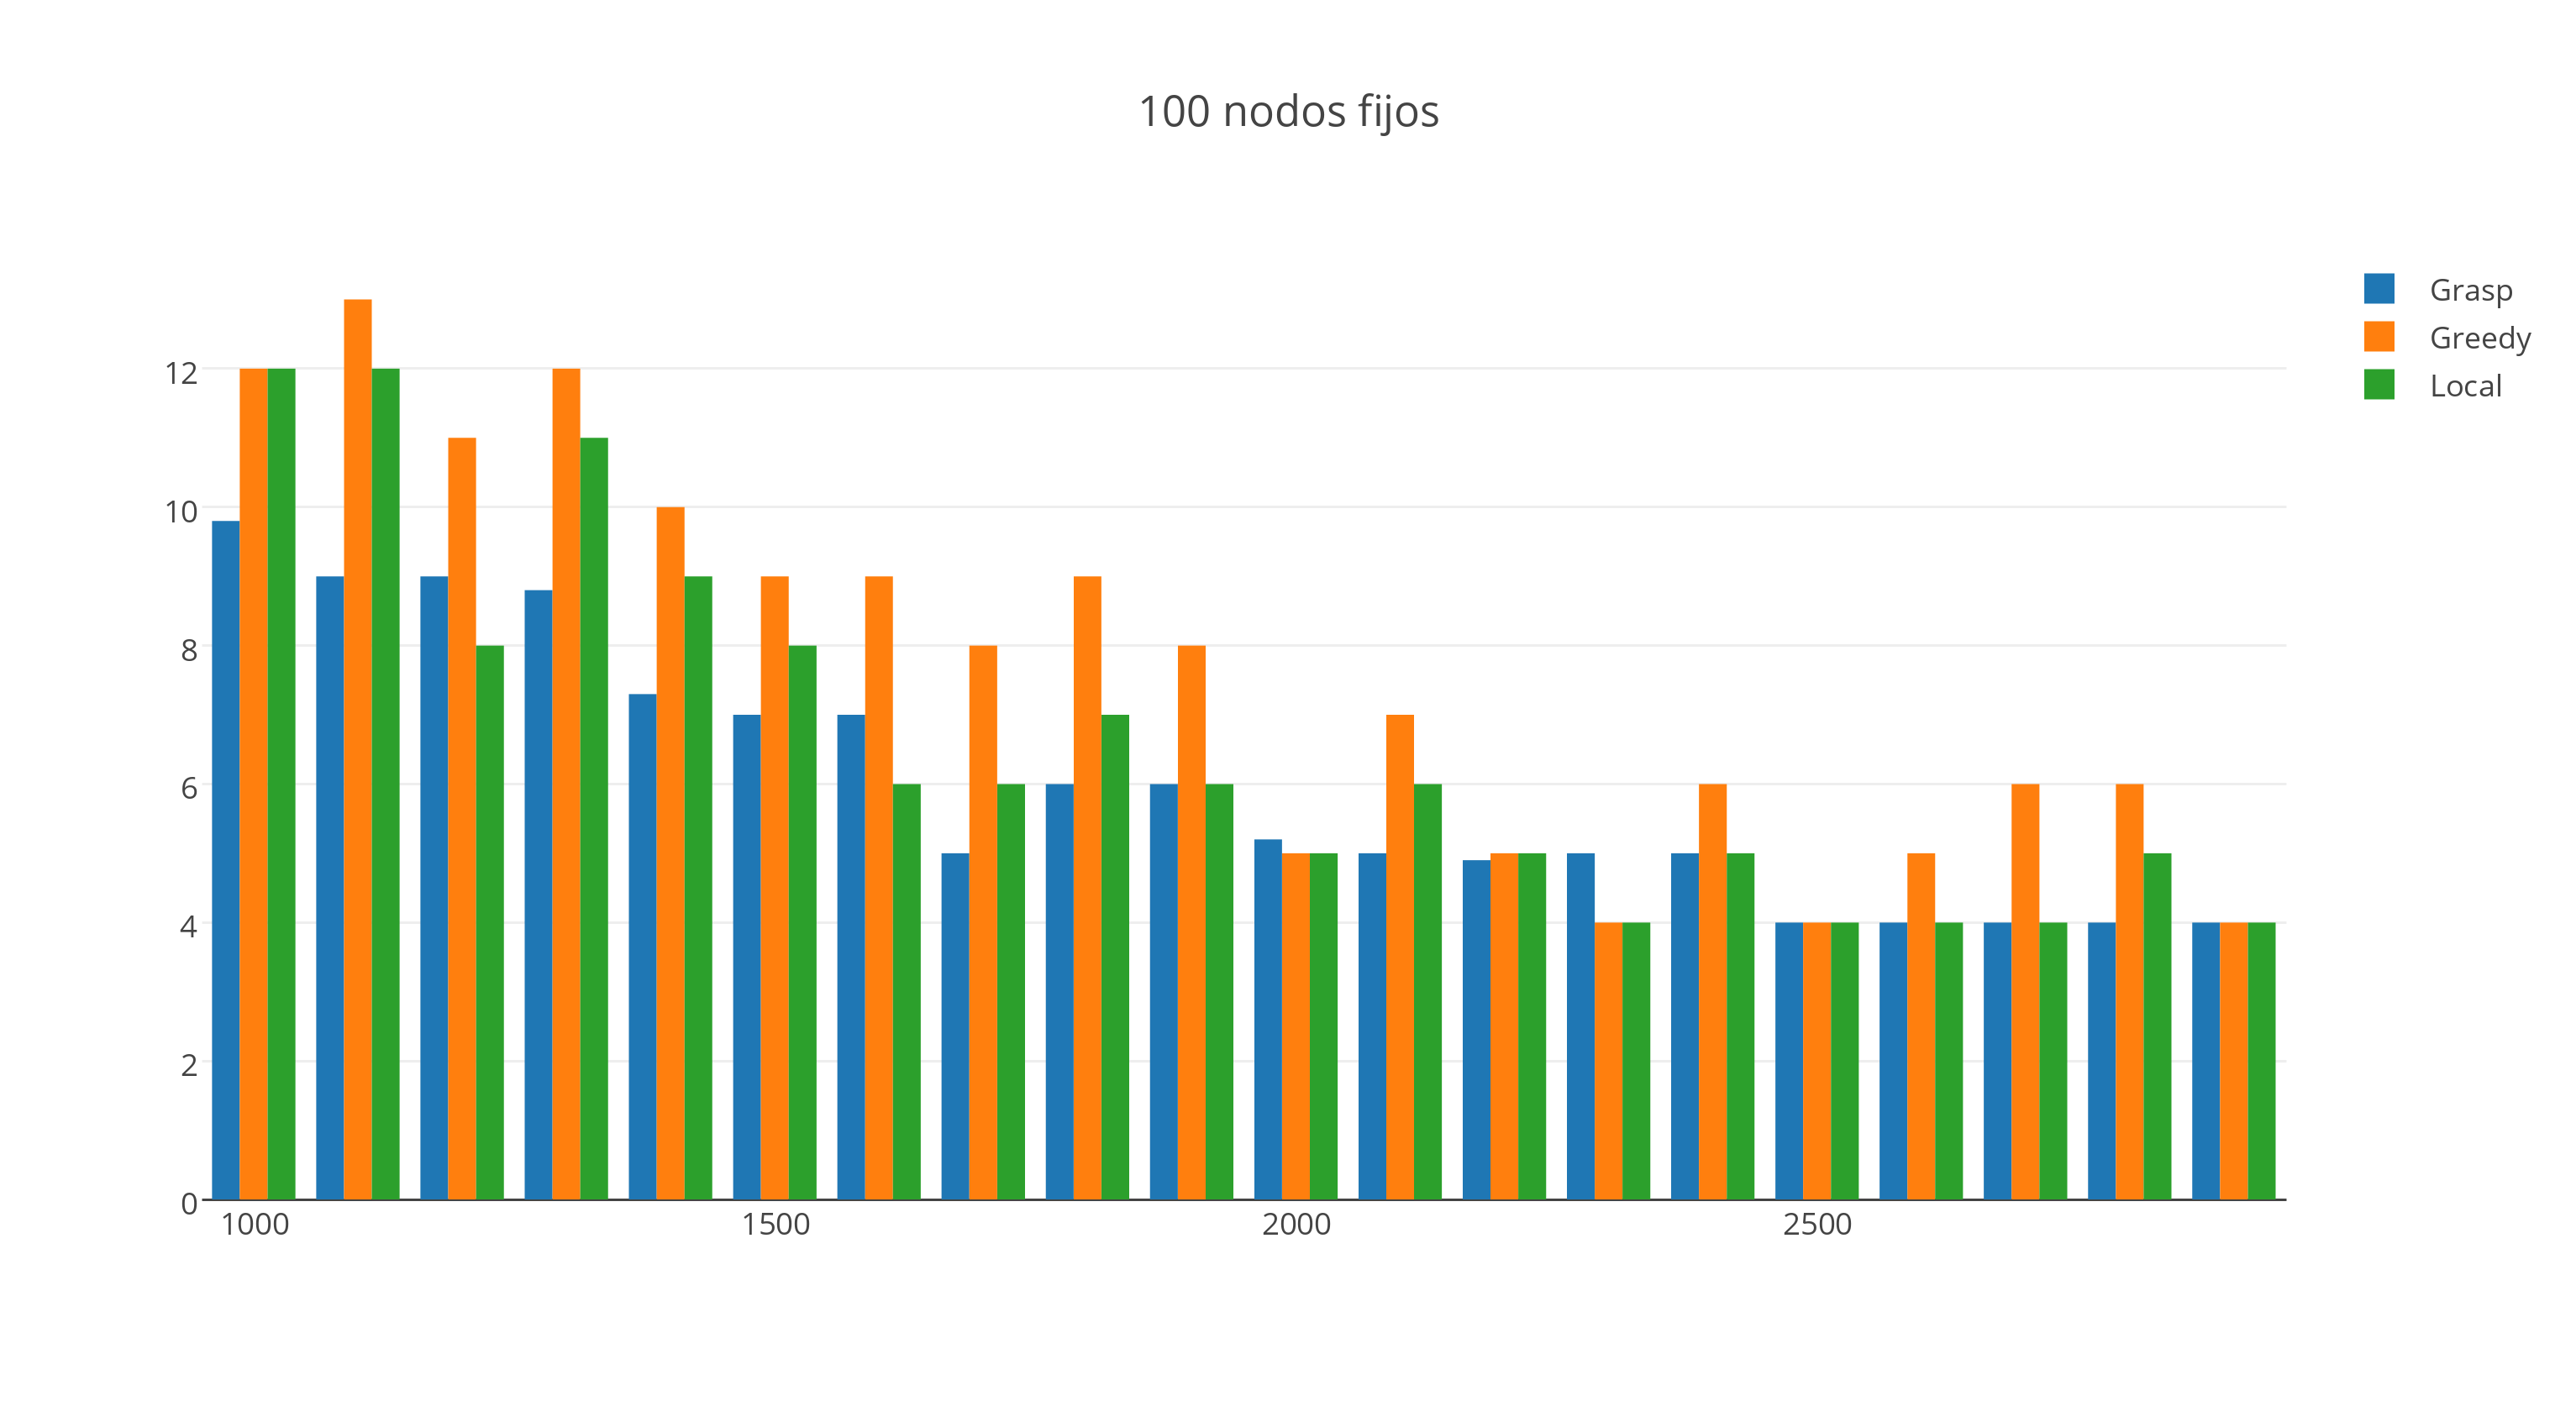
\includegraphics[width=13cm, keepaspectratio=yes]{imagenes/6/100NodosFijos.png}

 	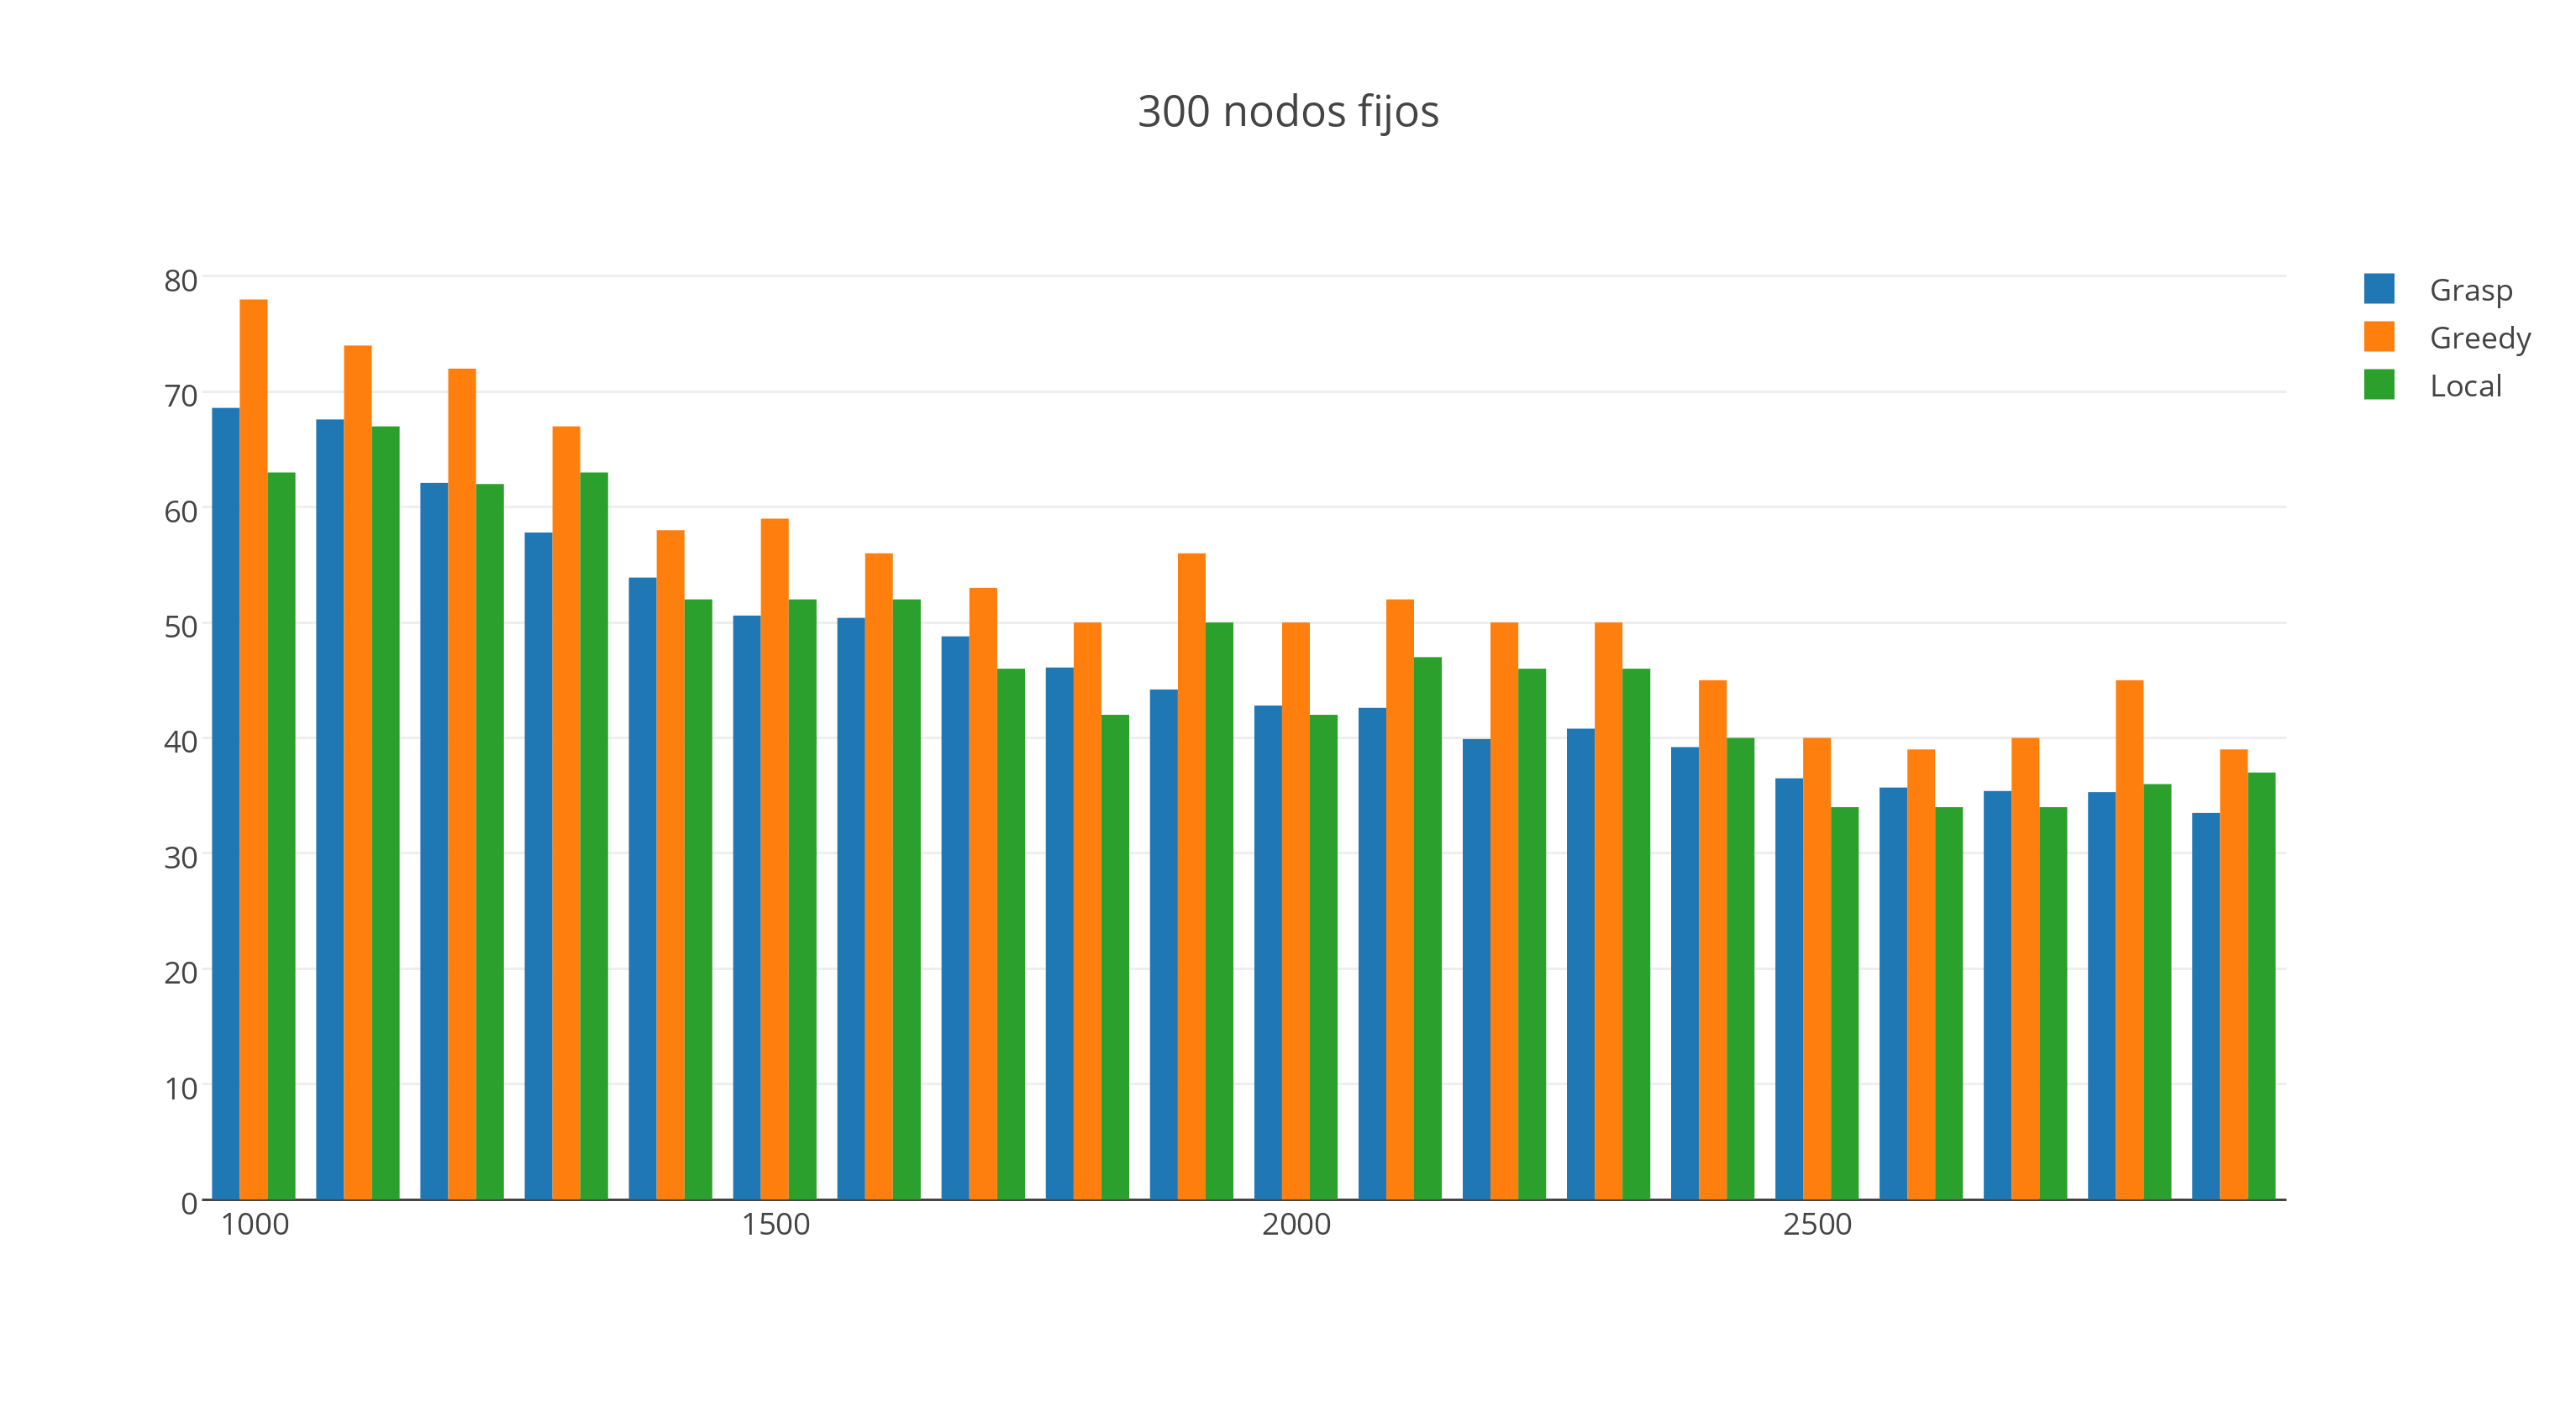
\includegraphics[width=13cm, keepaspectratio=yes]{imagenes/6/300NodosFijos.png}
 
 	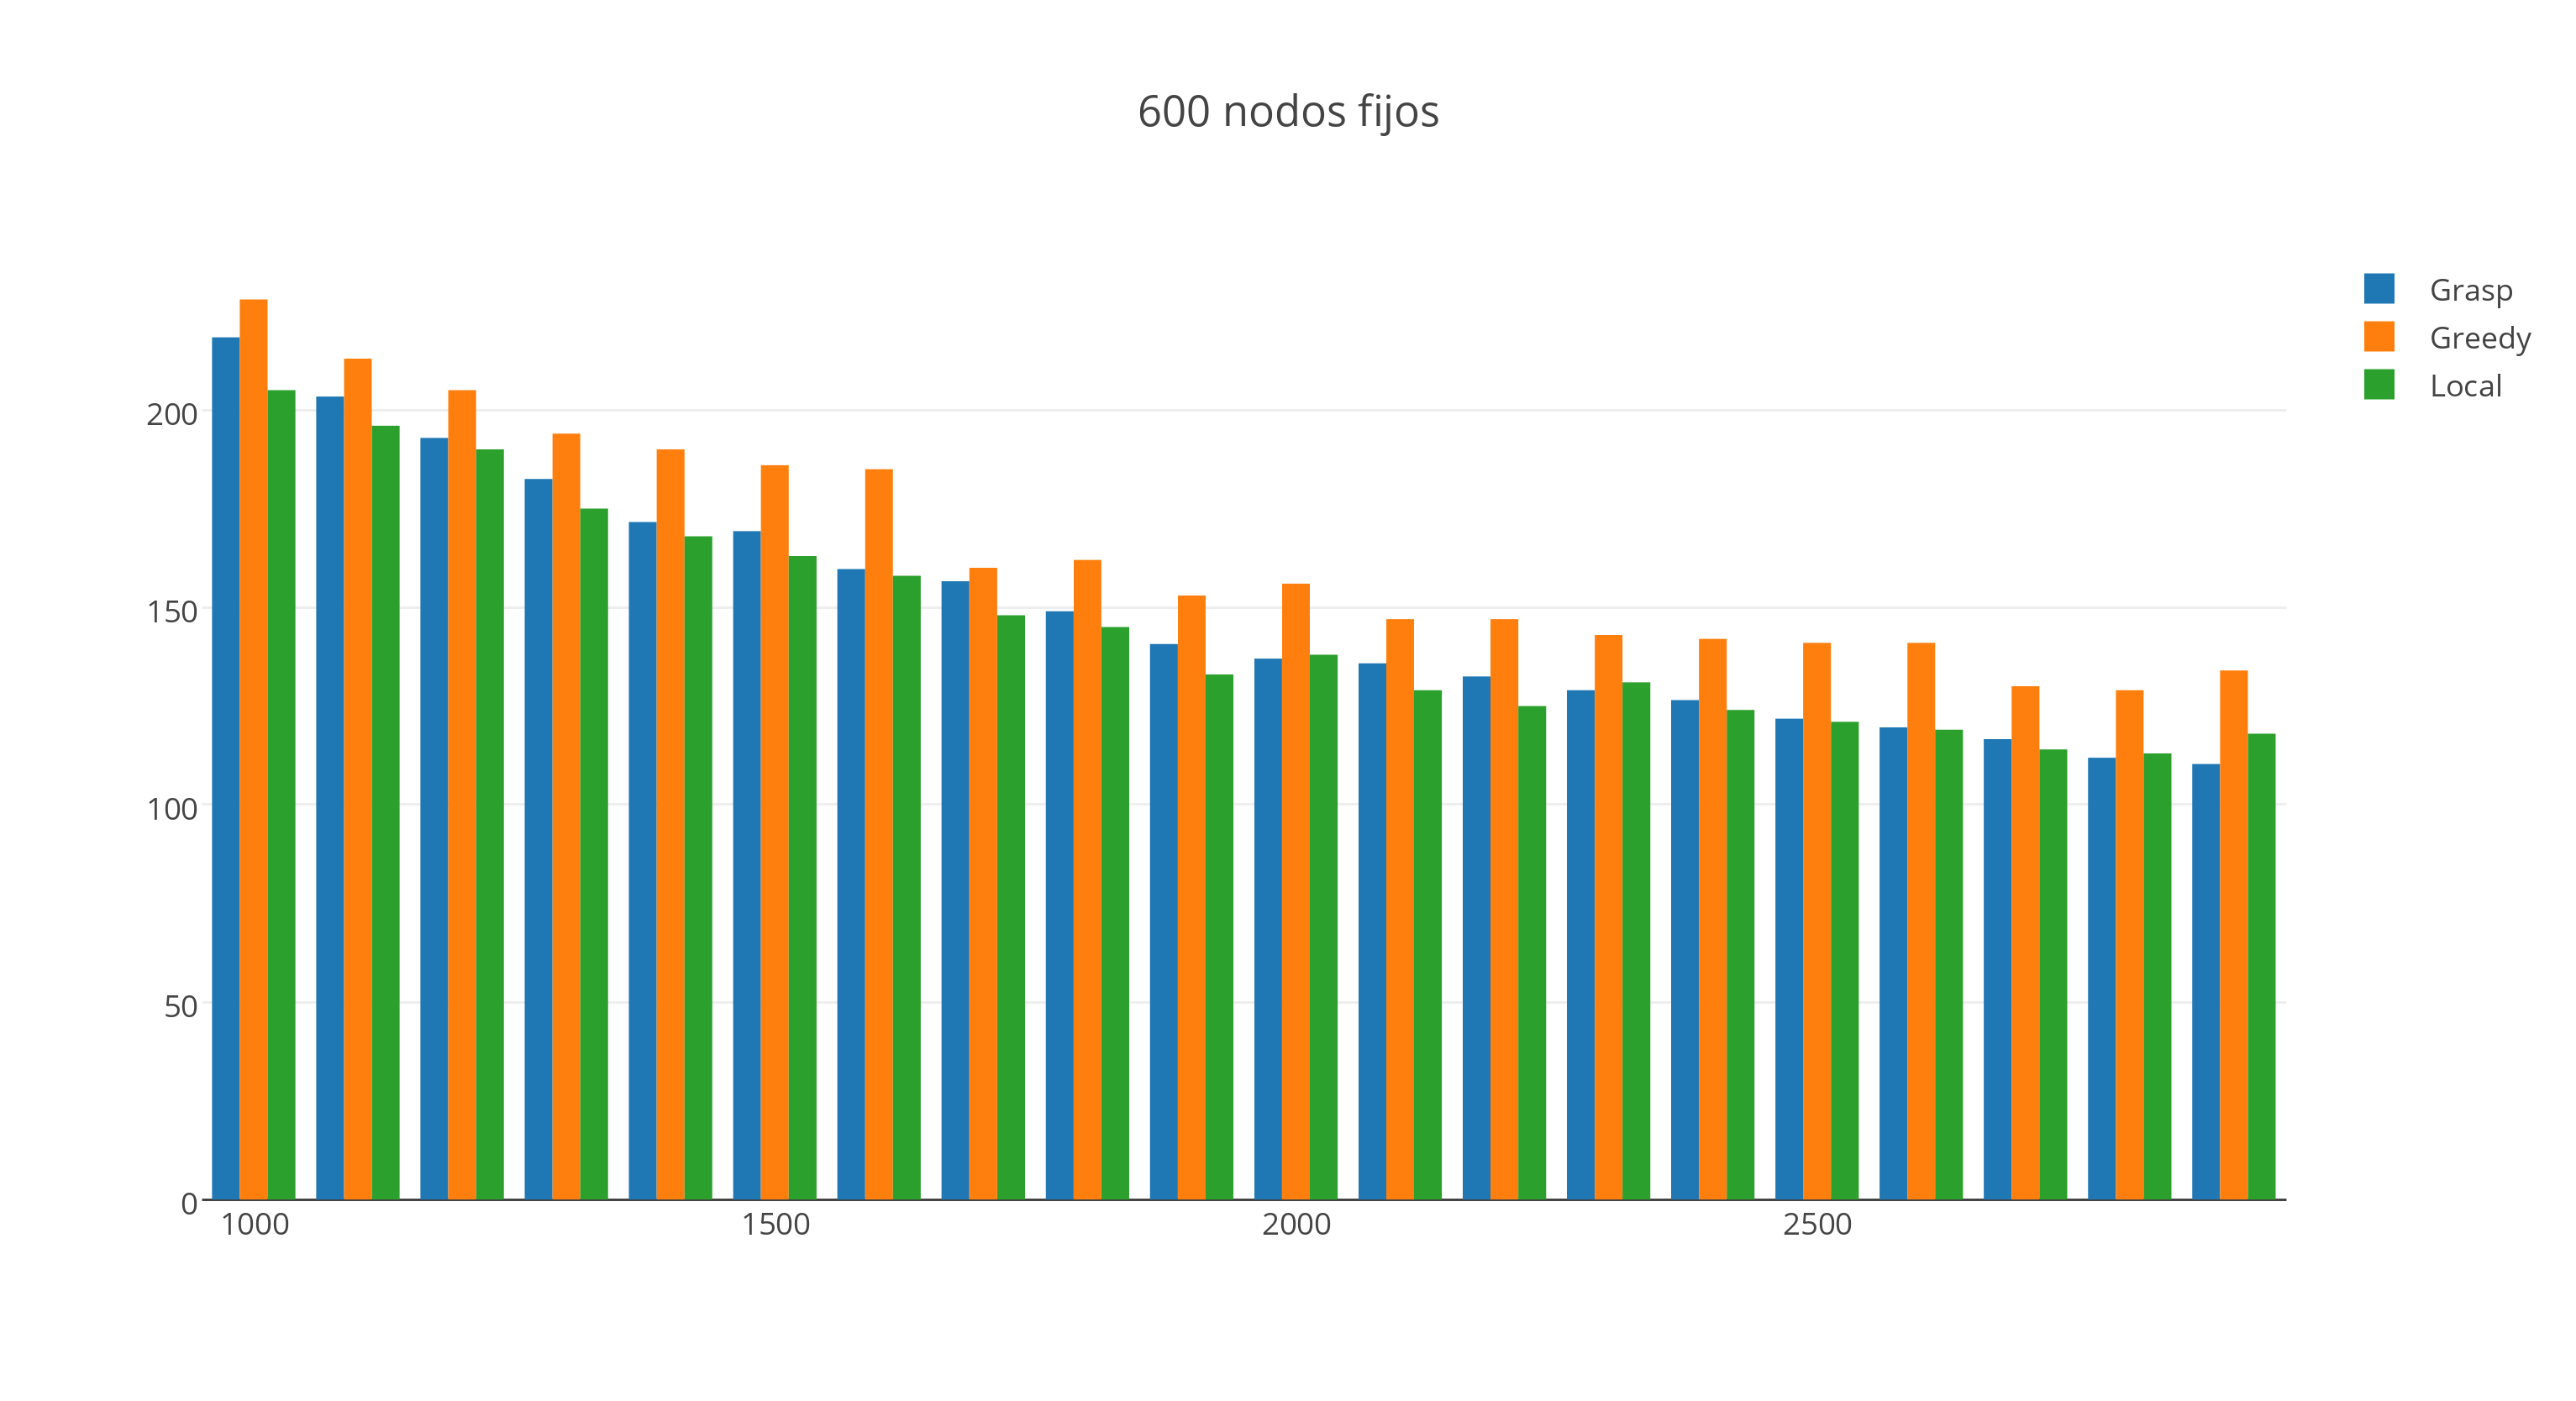
\includegraphics[width=13cm, keepaspectratio=yes]{imagenes/6/600NodosFijos.png}
 
 	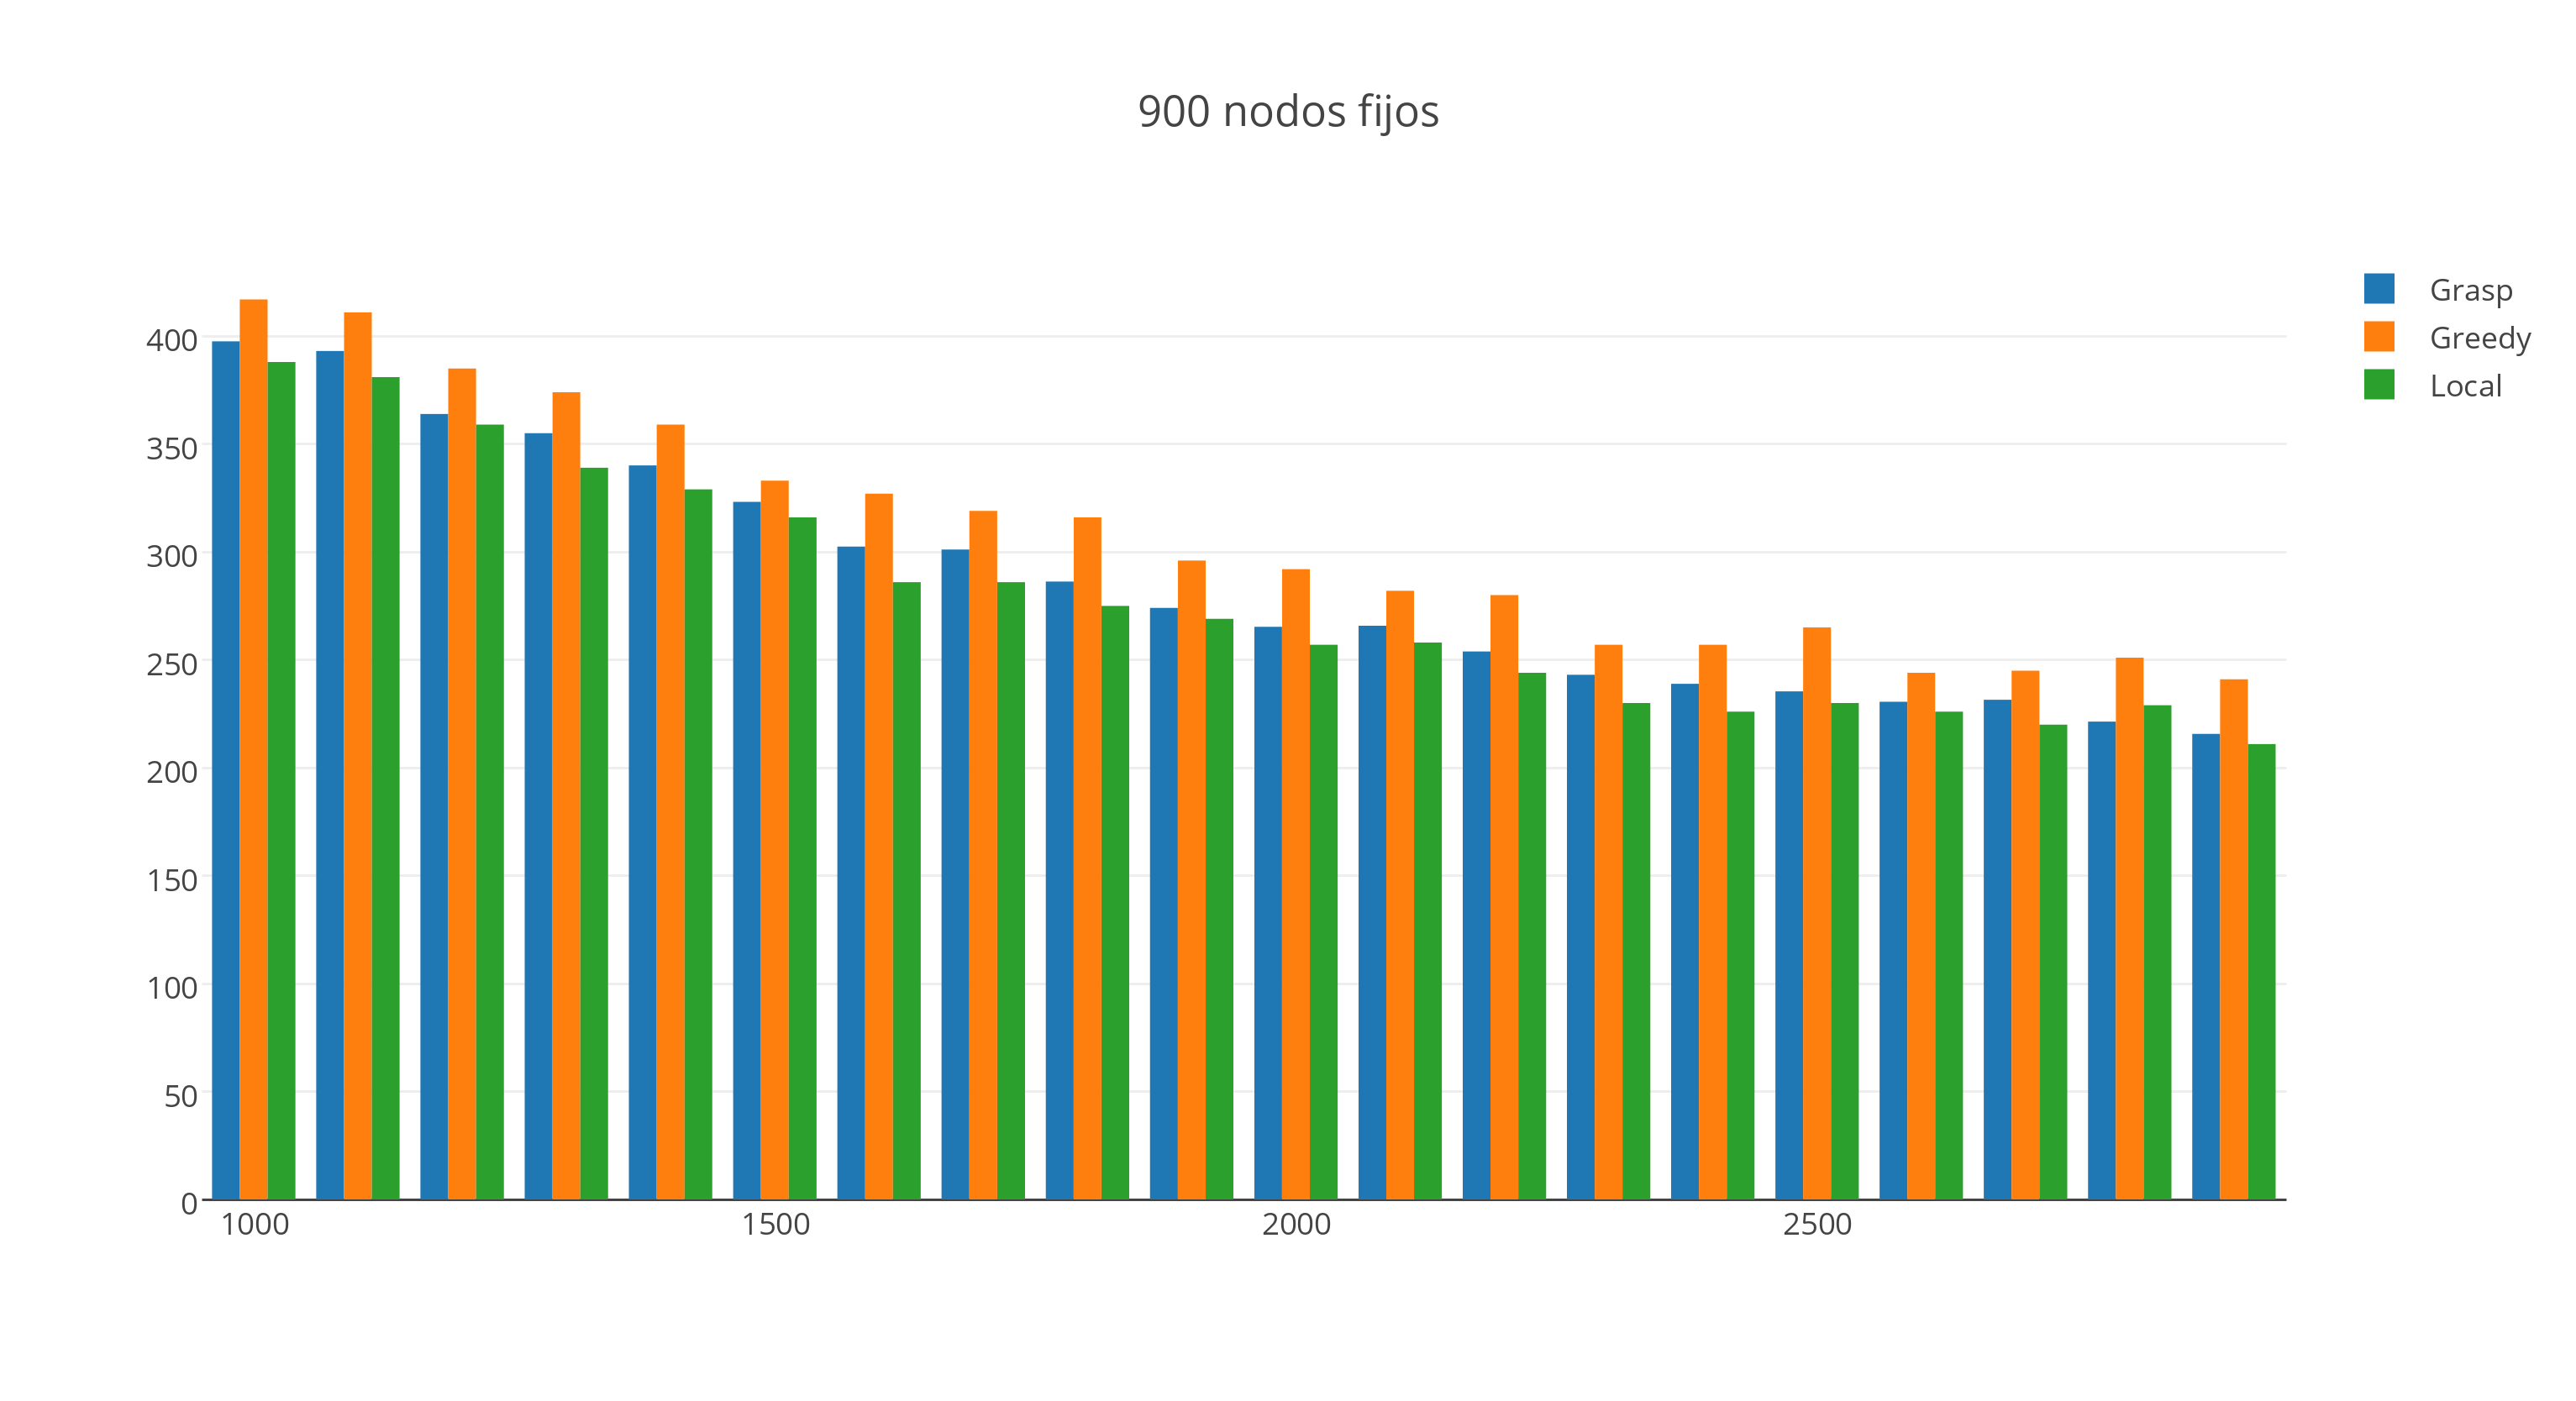
\includegraphics[width=13cm, keepaspectratio=yes]{imagenes/6/900NodosFijos.png}
\end{center}
 
Analizando estos gr\'aficos, podemos ver r\'apidamente que el algoritmo Greedy nos devuelve en todos los casos una soluci\'on peor que los otros dos, ya que utiliza mayor cantidad de nodos.\\
Por otra parte, se puede ver cierta ventaja del Grasp para los casos m\'as chicos (100, 300 nodos), pero para los casos grandes (600, 900 nodos), se ve que el Local es mejor en casi todos los casos.\\

No podemos distinguir claramente cu\'al es la mejor opci\'on entre estos dos, ya que los valores son bastante cambiantes a lo largo de los 4 gr\'aficos, por lo que buscamos el promedio de nodos que utiliza
cada algoritmo. Los resultados fueron los siguientes:\\

\textcolor{red}{Tabla con promedios}

Estos promedios confirman los datos que se pod\'ian apreciar en los gr\'aficos, es decir, que el Greedy utiliza siempre mayor cantidad de nodos que los otros, que Grasp es mejor en los casos chicos y
que a medida que crece la cantidad de nodos, es preferible el Local.\\

También se analizaron los tiempos de ejecución en las mismas instancias, cuyos resultados fueron los siguientes:

\begin{center}
 	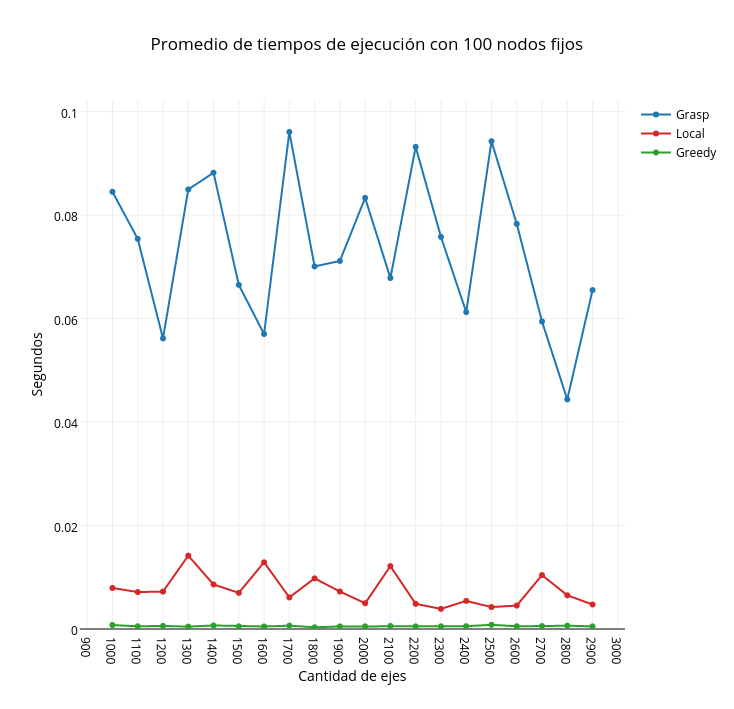
\includegraphics[width=13cm, keepaspectratio=yes]{imagenes/coliseo/Fixnode/100.png}

 	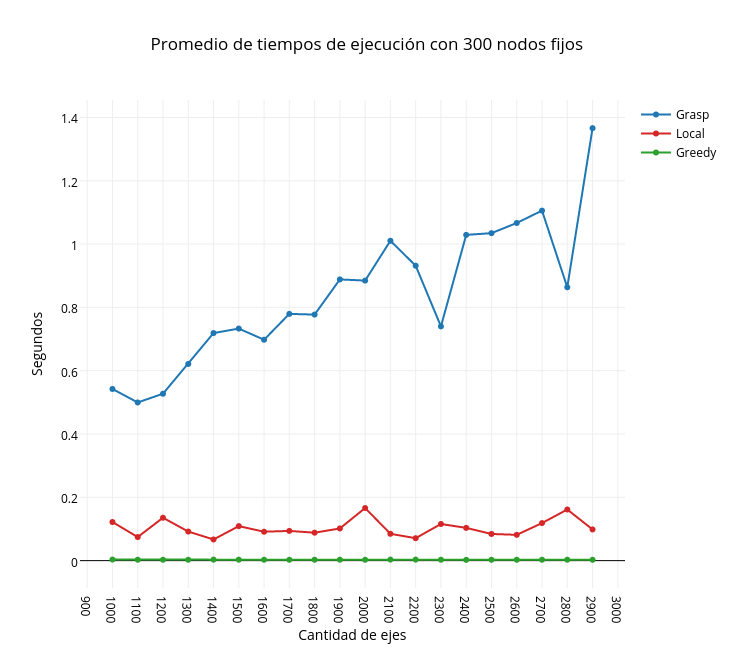
\includegraphics[width=13cm, keepaspectratio=yes]{imagenes/coliseo/Fixnode/300.png}

 	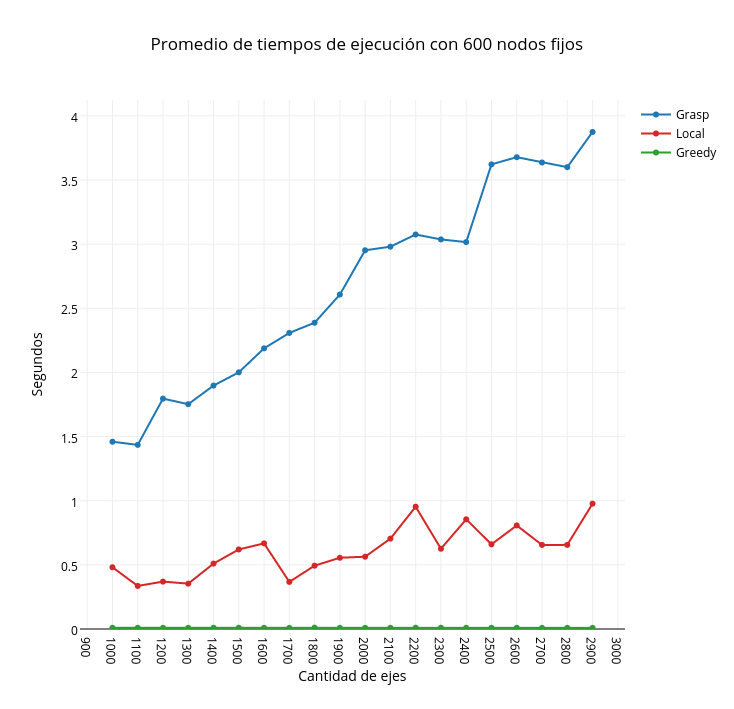
\includegraphics[width=13cm, keepaspectratio=yes]{imagenes/coliseo/Fixnode/600.png}

 	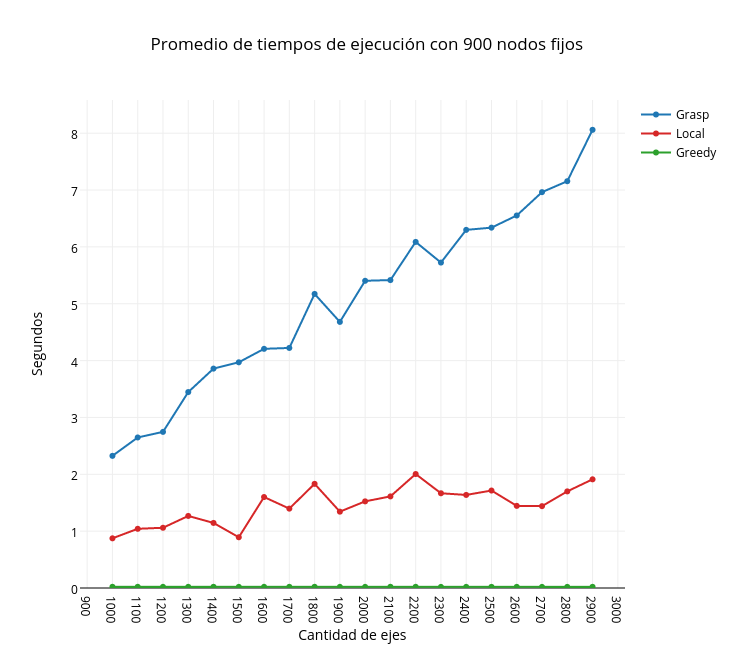
\includegraphics[width=13cm, keepaspectratio=yes]{imagenes/coliseo/Fixnode/900.png}
\end{center}

Se puede observar, que los algoritmos empeoran a mayor cantidad de nodos, pero debe notarse, que en general, Local y Greedy permanecen más bien constantes, mientras que Grasp empeora a mayor cantidad de ejes tiene, en grafos más grandes. 
Por lo tanto, y conforme al análisis anterior, queda aún más claro que para casos grandes, Local es la mejor alternativa al momento de fijar nodos y variar ejes, sea por tiempos de ejecución, como por mejor resultado.

\subsubsection{Ejes Fijos}
Para continuar, realizamos los mismos tests, pero manteniendo los ejes fijos y variando la cantidad de nodos. Los tests realizados fueron con ejes fijos desde 0 hasta 1000 y para cada instancia,
los nodos var\'ian de 50 a 1000.\\

Mostraremos los resultados obtenidos con 300, 600 y 900 ejes fijos:\\

   \begin{center}
 	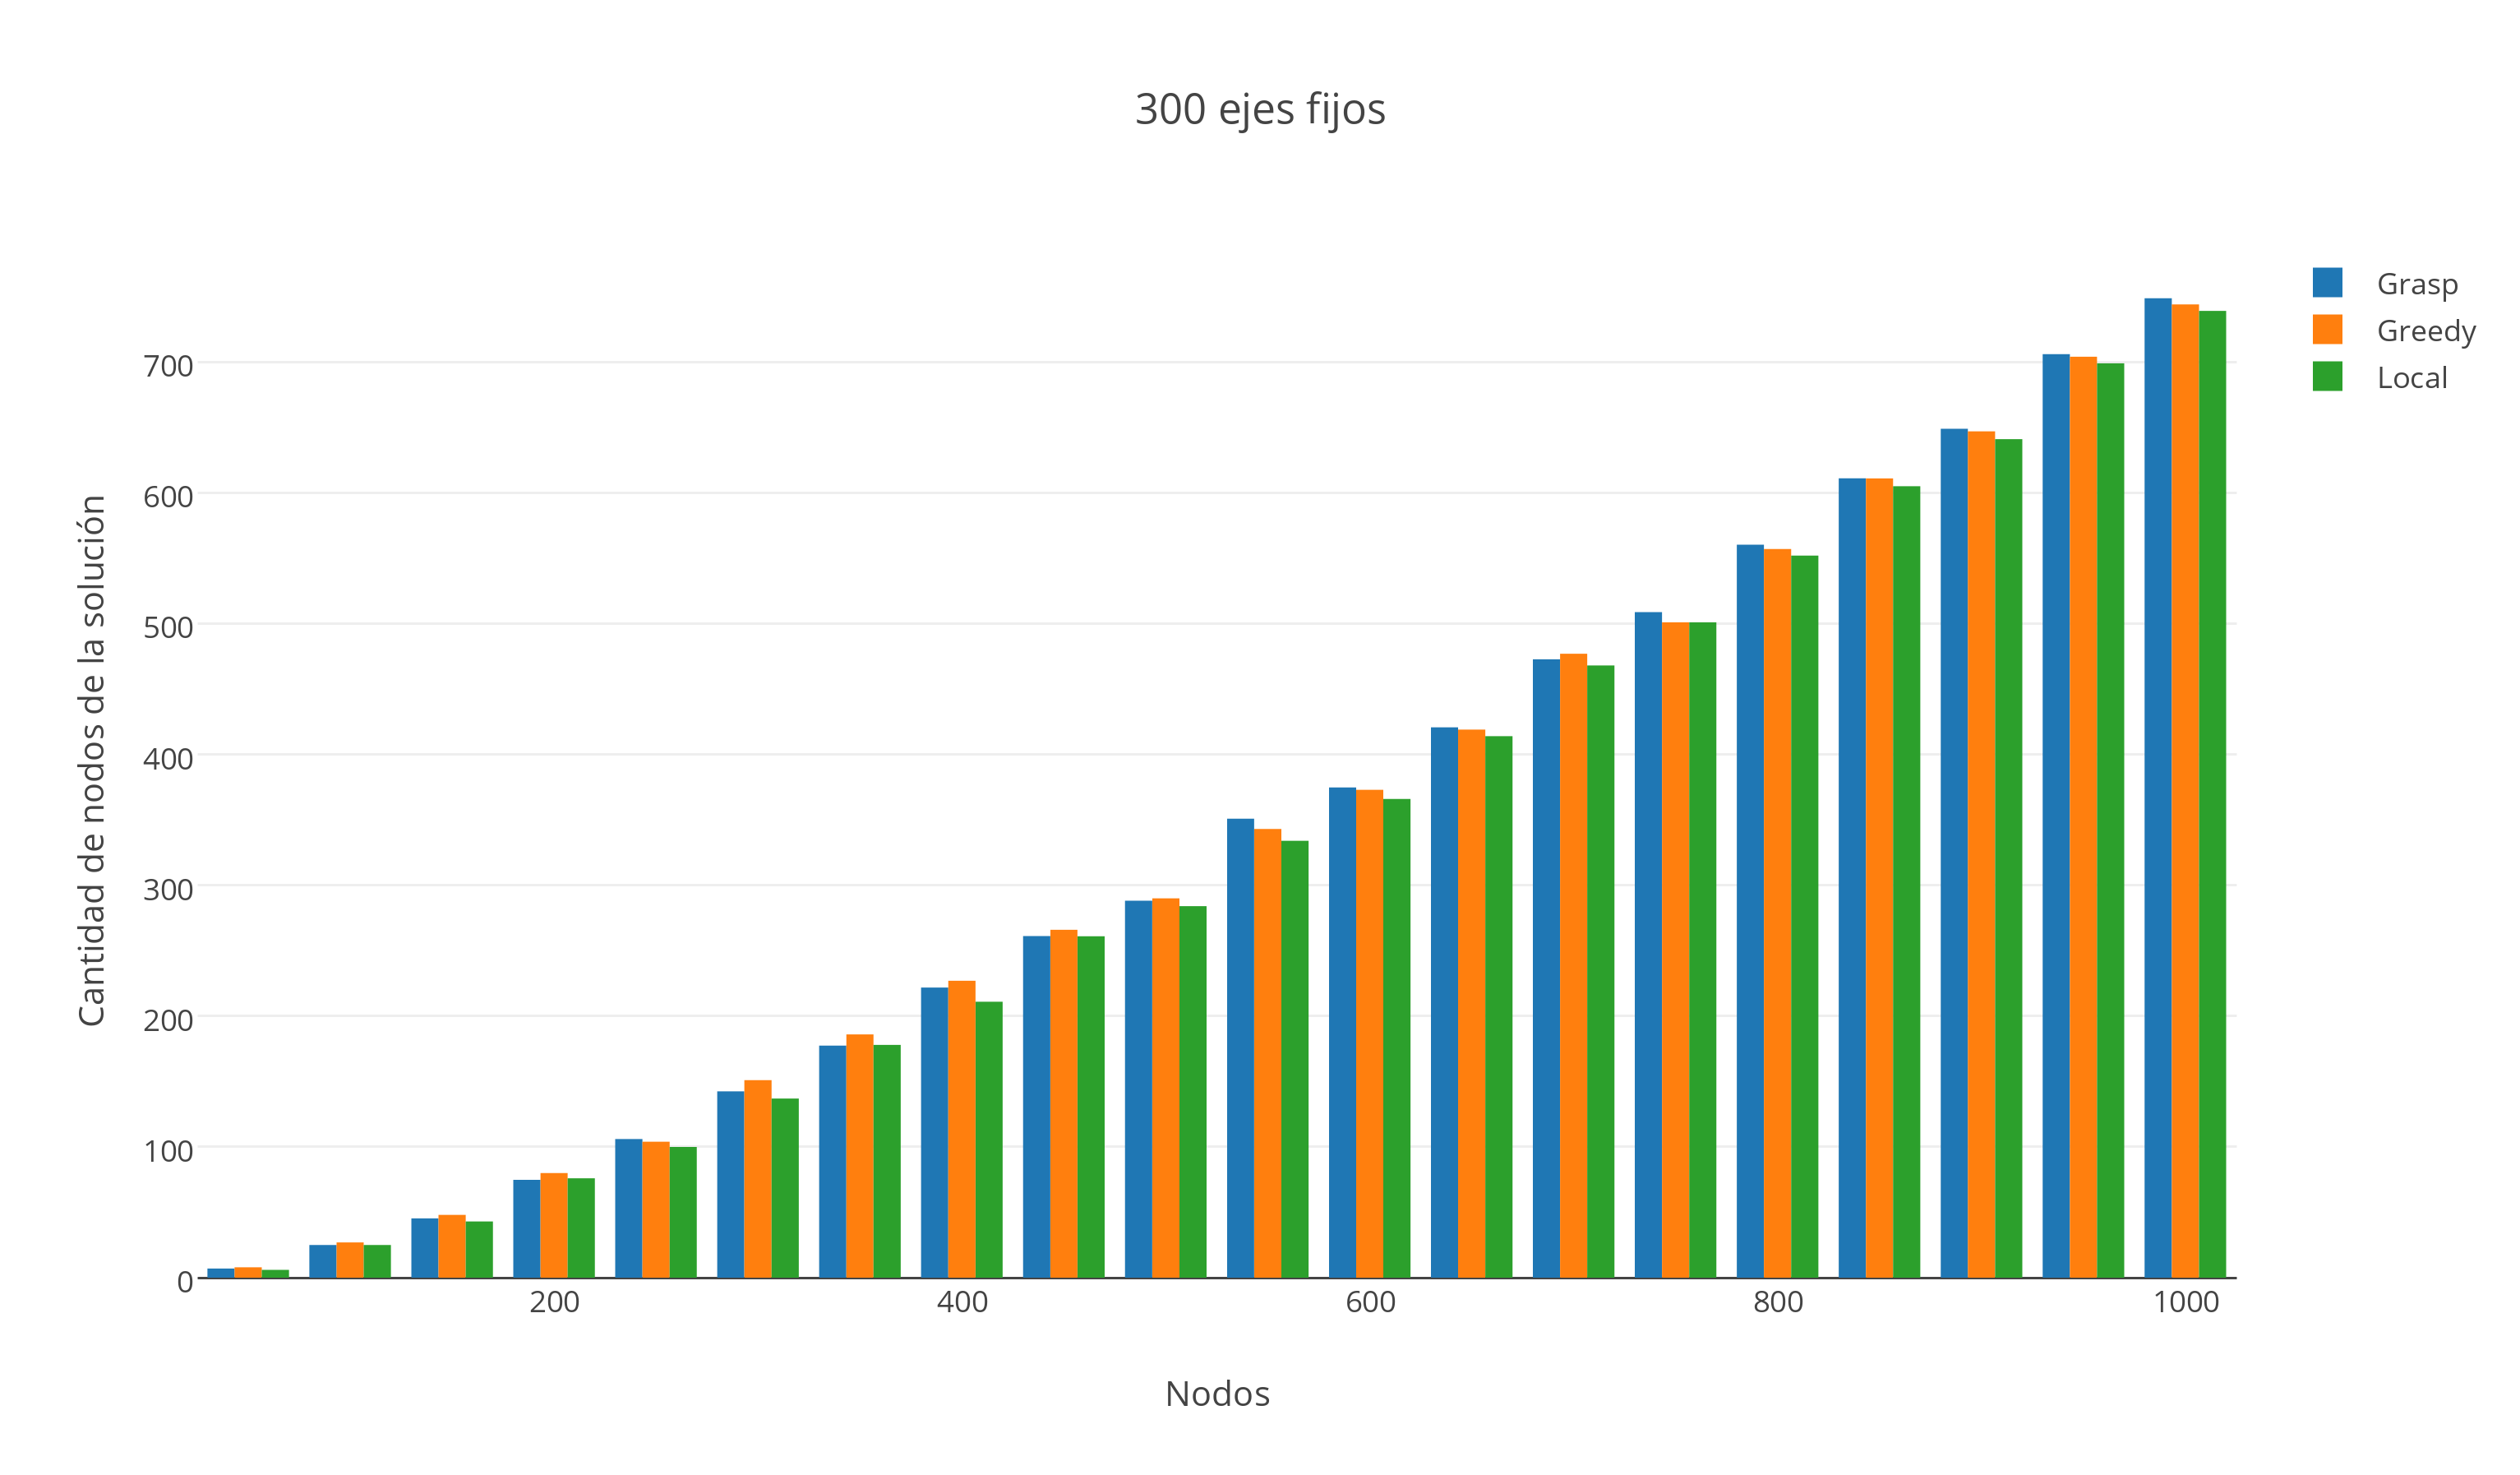
\includegraphics[width=13cm, keepaspectratio=yes]{imagenes/6/300EjesFijos.png}

 	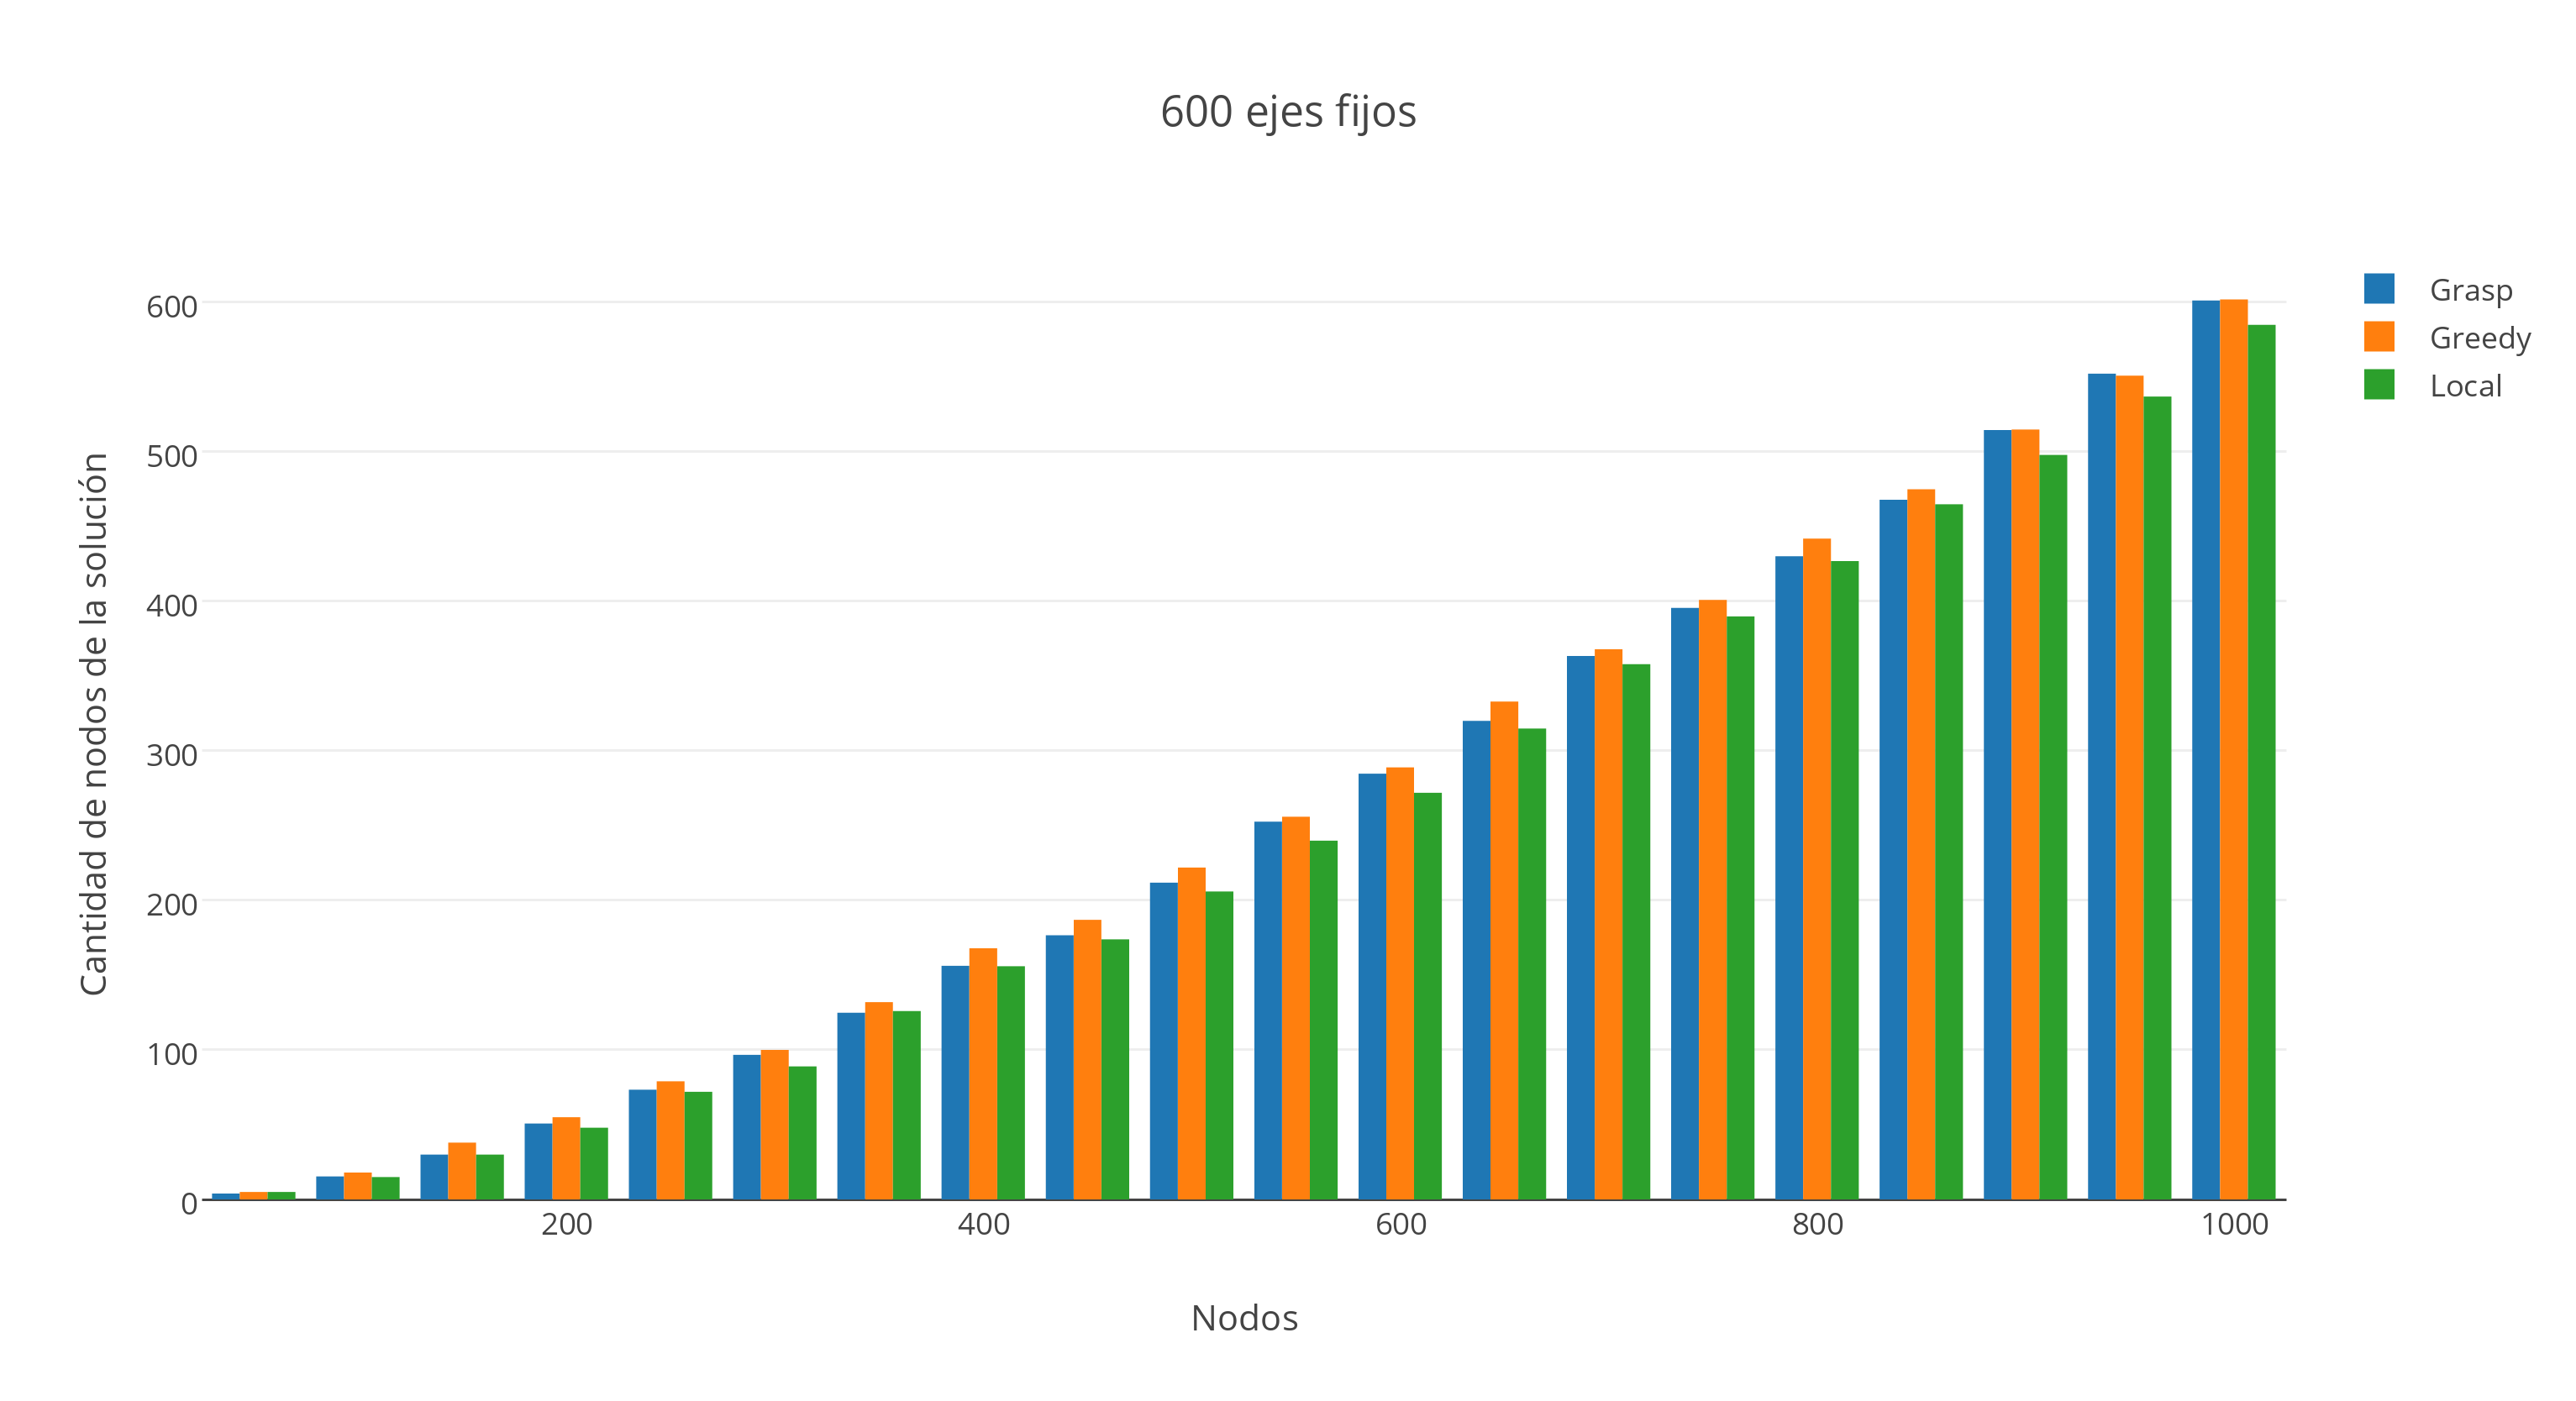
\includegraphics[width=13cm, keepaspectratio=yes]{imagenes/6/600EjesFijos.png}

 	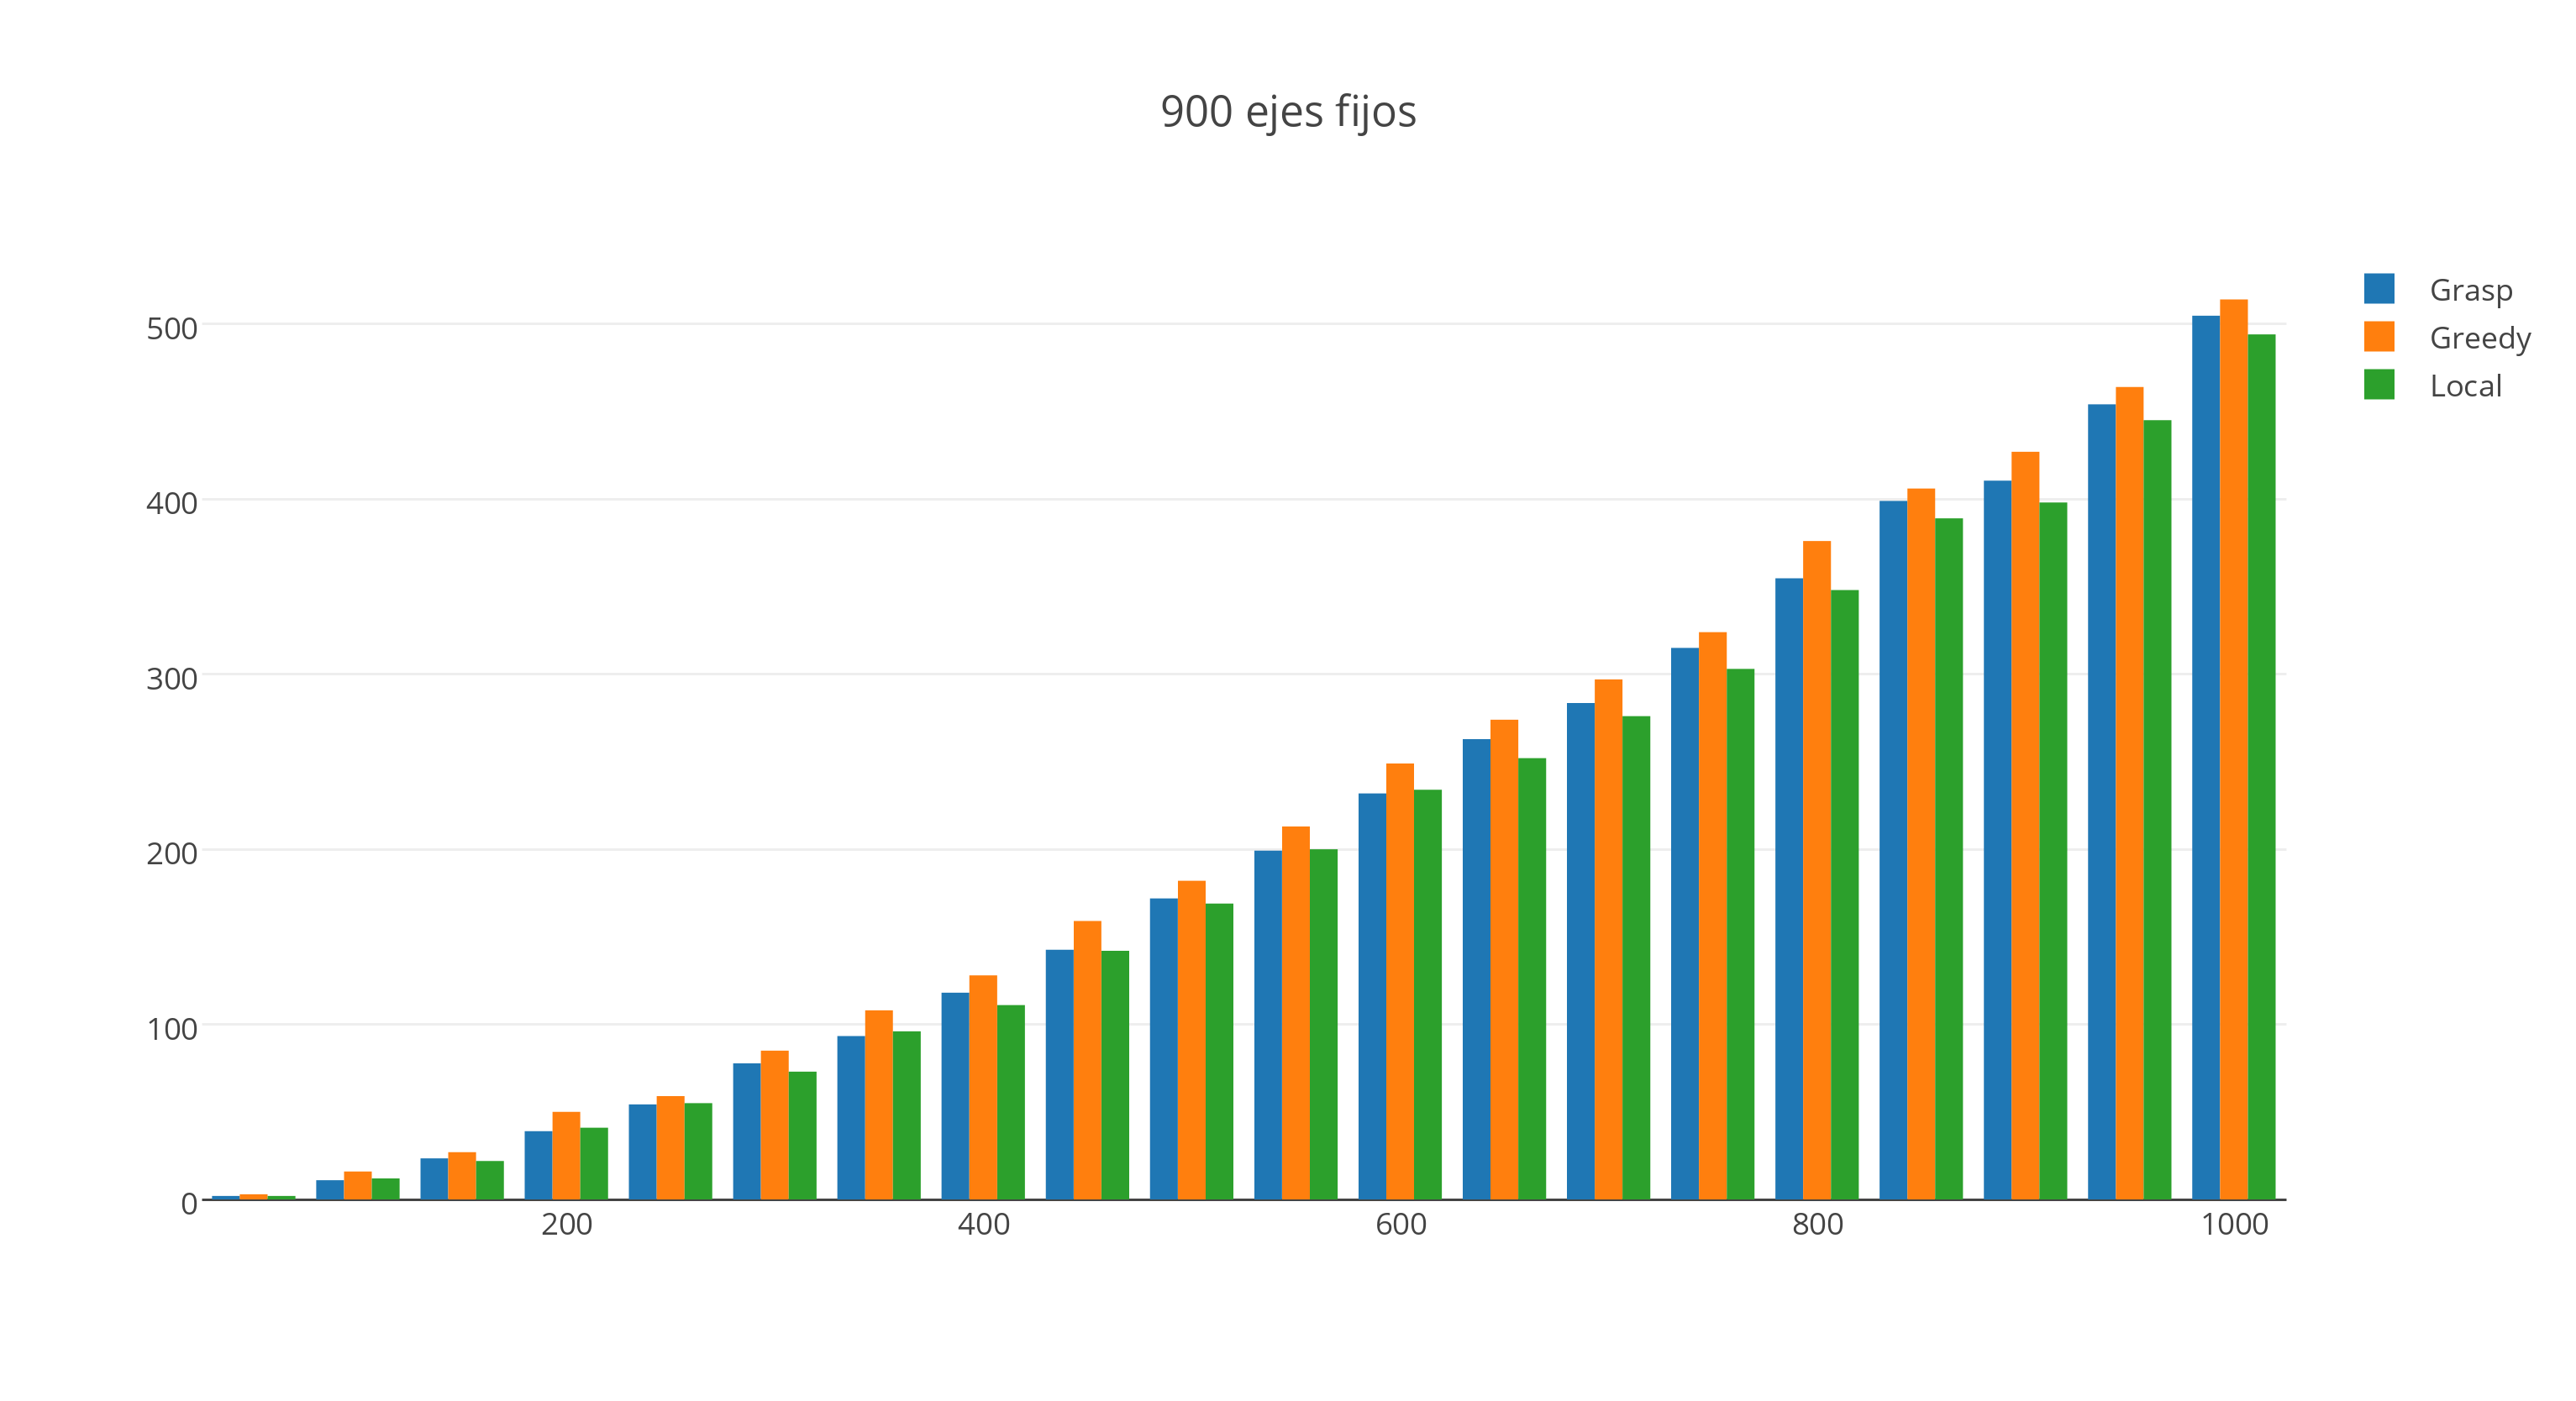
\includegraphics[width=13cm, keepaspectratio=yes]{imagenes/6/900EjesFijos.png}
   \end{center}
 
A primera vista, se puede ver que para casi todas las instancias el algoritmo de B\'usqueda Local es el que menos nodos utiliza en su soluci\'on. 
En cuanto al Greedy y el Grasp, las diferencias son chicas y alternadas con 300 ejes, pero con 600 y 900 ejes, Greedy aparenta ser el peor.\\

Para corroborar estos datos, tomamos nuevamente el promedio de todas las soluciones:\\

\textcolor{red}{Tabla con promedios}

Como preve\'iamos, estos promedios confirman nuestro an\'alisis.

Nuevamente, para fortalecer nuestra conclusión, se analizaron los tiempos de ejecución en las mismas instancias, cuyos resultados fueron los siguientes:

\begin{center}
 	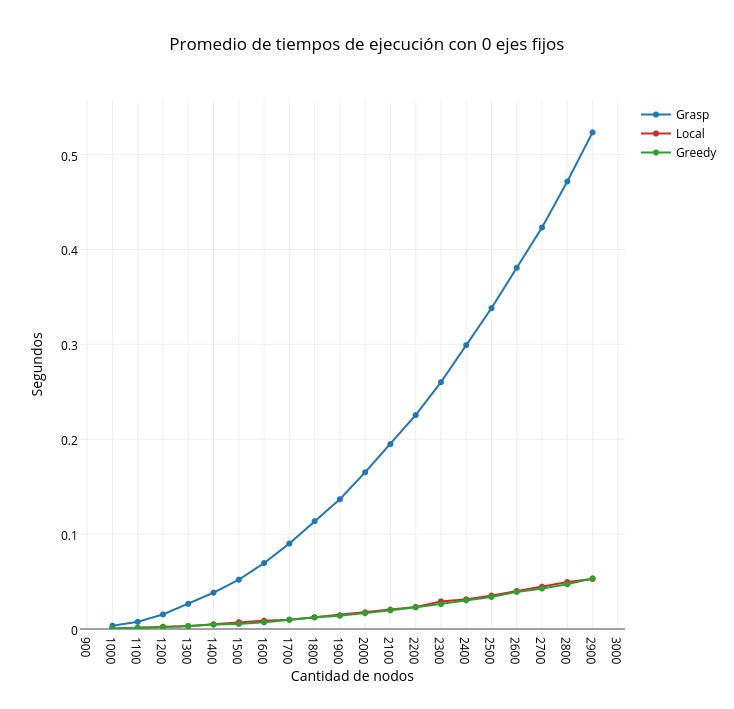
\includegraphics[width=13cm, keepaspectratio=yes]{imagenes/coliseo/Fixedge/0.png}

 	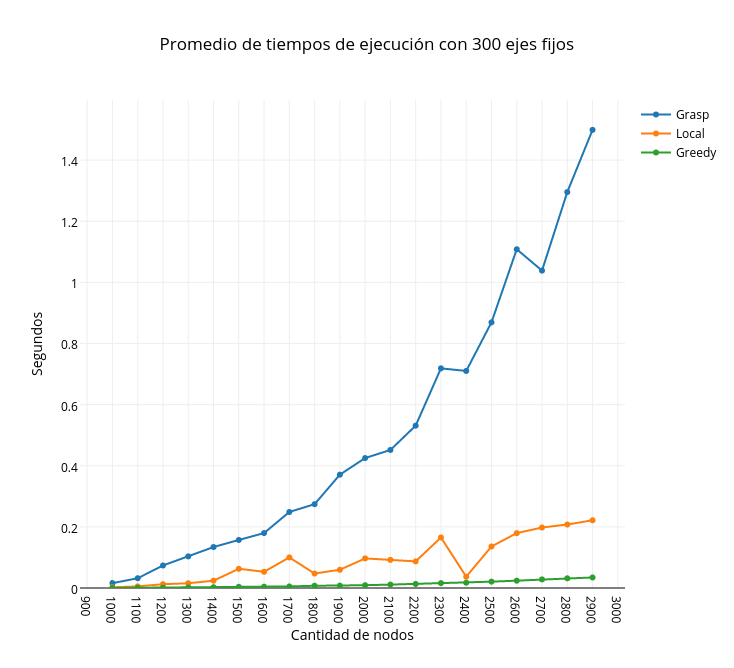
\includegraphics[width=13cm, keepaspectratio=yes]{imagenes/coliseo/Fixedge/300.png}

 	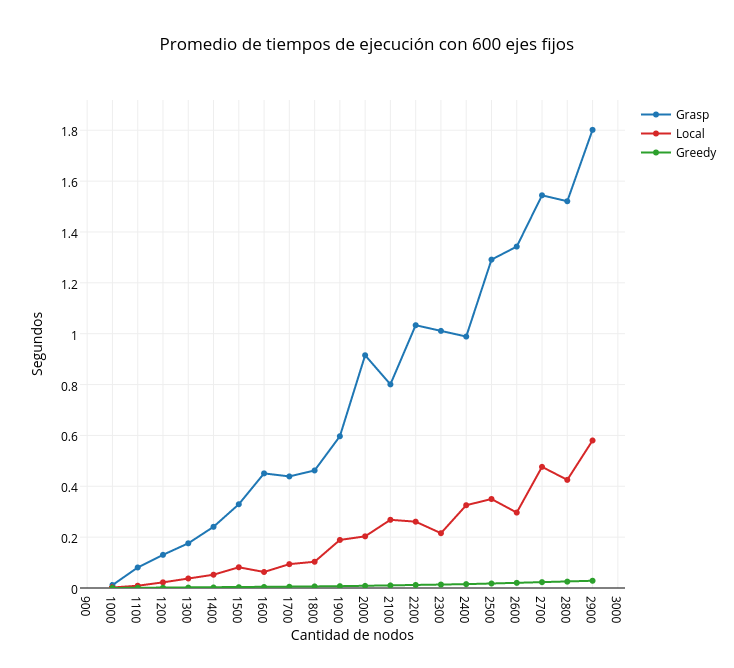
\includegraphics[width=13cm, keepaspectratio=yes]{imagenes/coliseo/Fixedge/600.png}

 	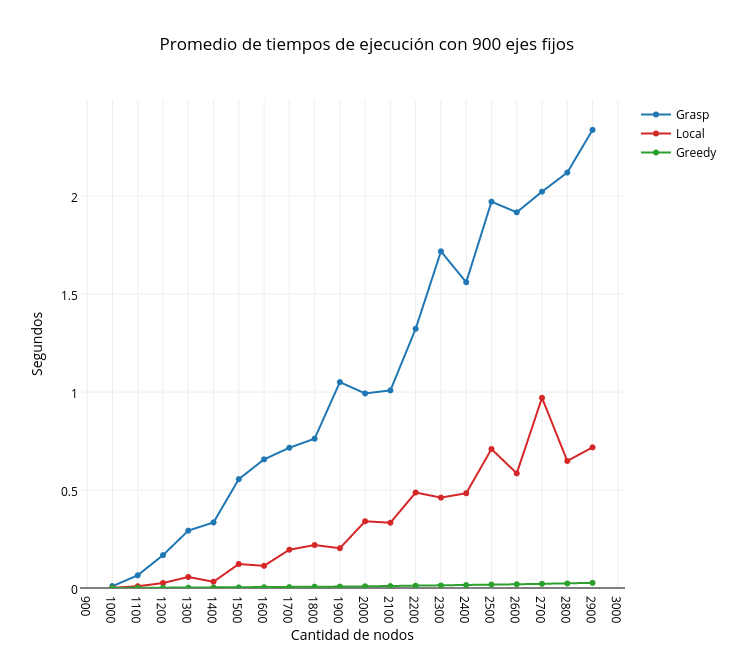
\includegraphics[width=13cm, keepaspectratio=yes]{imagenes/coliseo/Fixedge/900.png}
\end{center}

Como era esperado, Grasp insume mayor tiempo que Local y Greedy para cualquier caso.
Considerando los resultados y los tiempos de ejecución, concluímos que Local es la mejor alternativa, si se mantienen ejes y se varían nodos.

\subsection{Familias específicas}
\subsubsection{Grafo completo}

\textcolor{red}{Diganme si vale la pena hablar sobre grafos completos. Onda, la respuesta es trivial, y los tiempos son meh}

\subsubsection{Grafo bipartito completo}

\textcolor{red}{Brian contandonos un poco los resultados del bipartito completo}

Analizando también los tiempos de ejecución sobre las mismas instancias, se obtuvieron los siguientes resultados:

\begin{center}
 	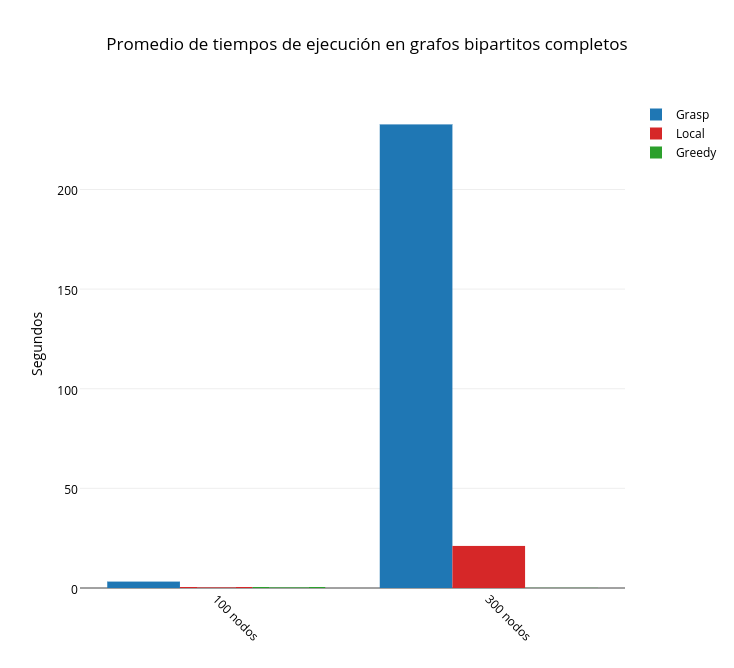
\includegraphics[width=13cm, keepaspectratio=yes]{imagenes/coliseo/Bipartite1.png}

 	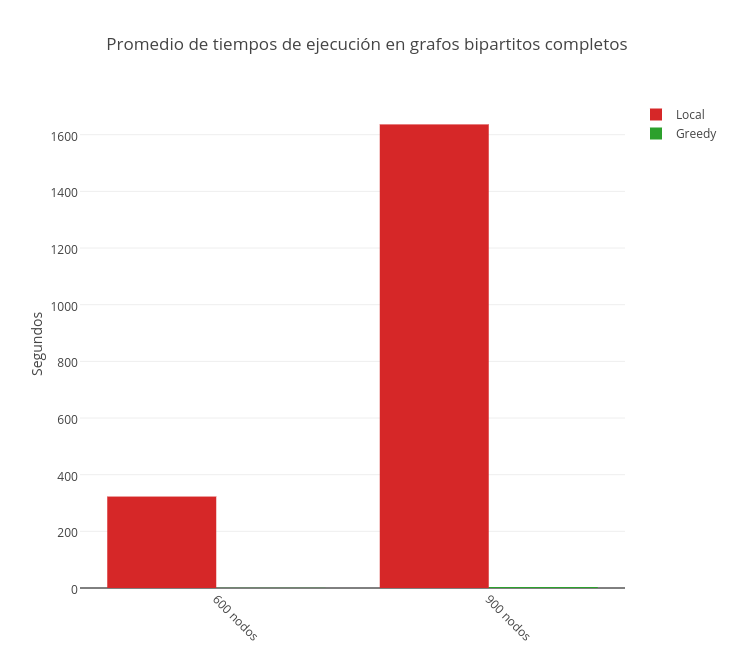
\includegraphics[width=13cm, keepaspectratio=yes]{imagenes/coliseo/Bipartite2.png}
\end{center}

<<<<<<< HEAD
Para el segundo gráfico, se omitió la ejecución del Grasp, dado que los tiempos de ejecución del mismo para los grafos bipartitos completos de esa magnitud, eran demasiado altos 
\textcolor{red}{Y Ezequiel nos cuenta como esto se debe a los pares de nodos que agarra}.
=======
Para el segundo gráfico, se omitió la ejecución del Grasp, dado que los tiempos de ejecución del mismo para los grafos bipartitos completos de esa magnitud, eran demasiado altos, esto era predecible, pues debe ejecutar la b\'usqueda local 10 veces, es decir que su ejecuci\'on consume \textit{10x(tiempo de b\'usqueda local)}.
>>>>>>> 8e16beb30cc5e5a85853803ffadc91069733de28

Dado que los tres algoritmos siempre obtienen la solución óptima para la familia de grafos bipartitos completos, concluímos que el Greedy es el mejor de los tres para estos casos, ya que es el que menor tiempo insume. 

\subsubsection{Ciclo simple}

\textcolor{red}{Brian contandonos un poco los resultados del ciclo simple}
Por \'ultimo, analizaremos qu\'e ocurre cuando el grafo de entrada es un ciclo. Para ello fuimos generando distintos ciclos, comenzando con 100 nodos y aumentando de a 100 hasta 1000 nodos.\\
Los resultados obtenidos fueron:\\

\begin{center}
 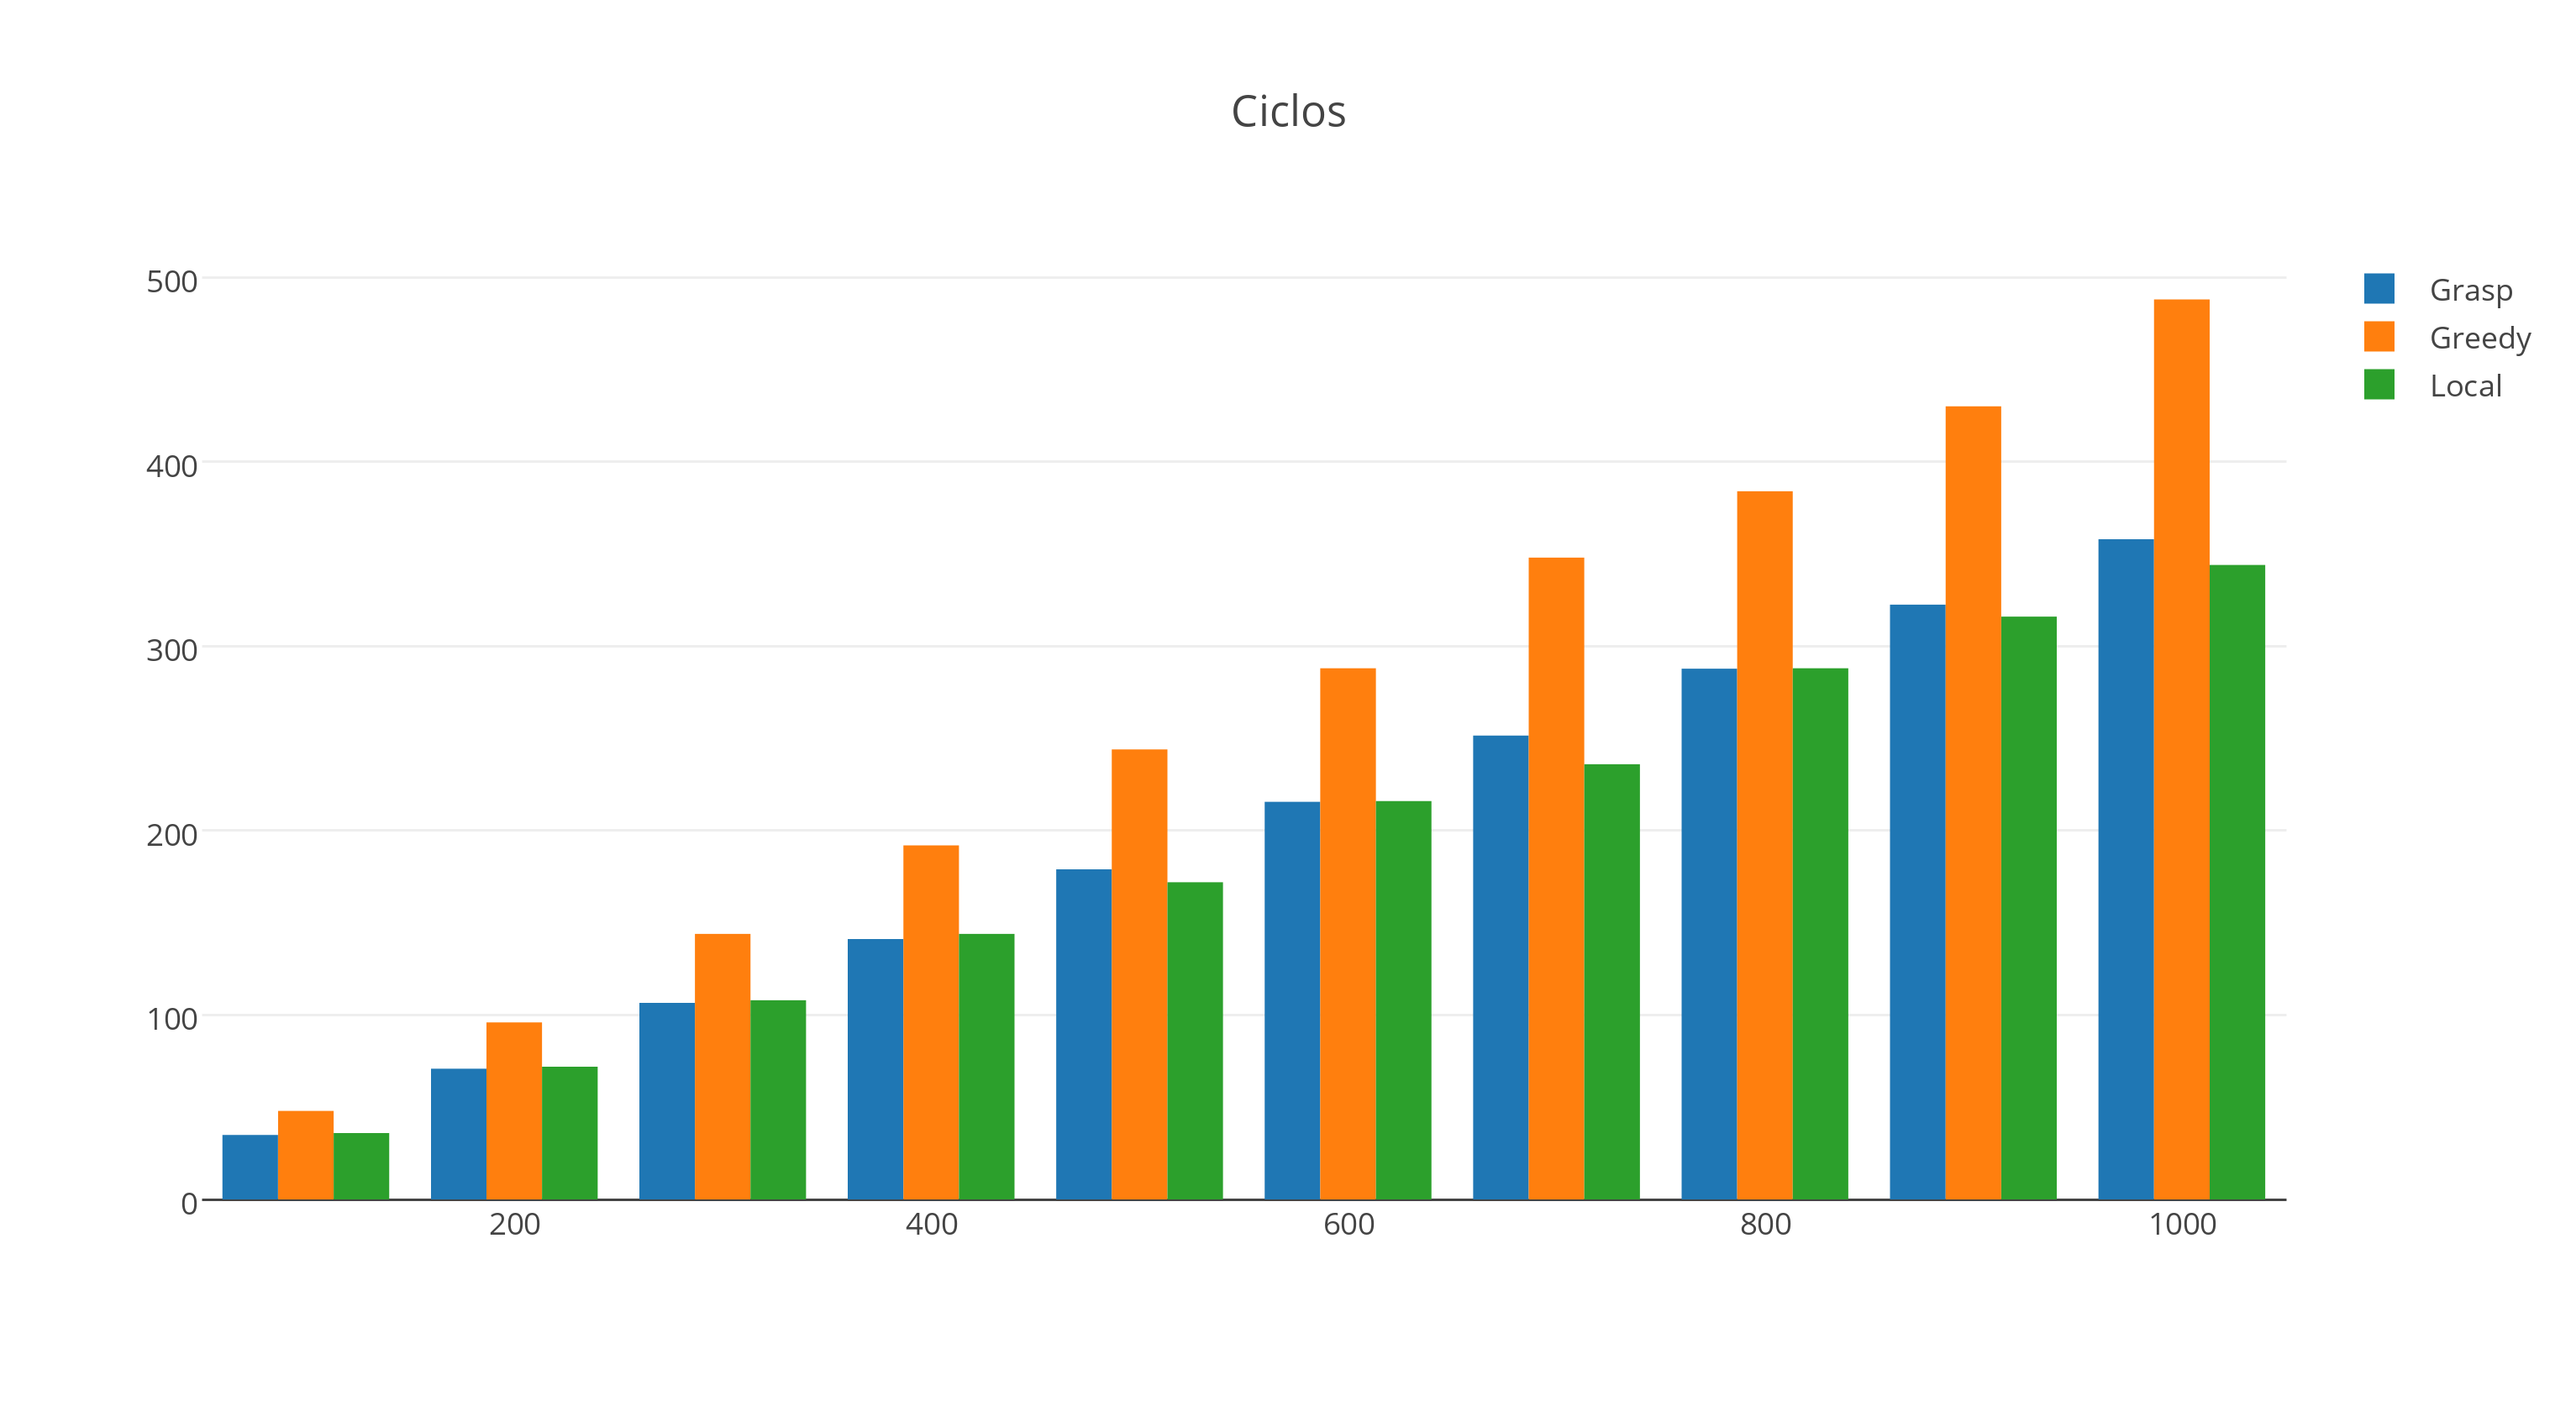
\includegraphics[width=13cm, keepaspectratio=yes]{imagenes/6/Ciclos.png}
\end{center}

Se aprecia r\'apidamente que el Greedy es el peor de los 3 y que los resultados entre el Grasp y Local son muy parejos, siendo Local un poco mejor en los casos m\'as grandes.\\

A su vez, los tiempos de ejecucion sobre las mismas instancias, se obtuvieron los siguientes resultados:

\begin{center}
 	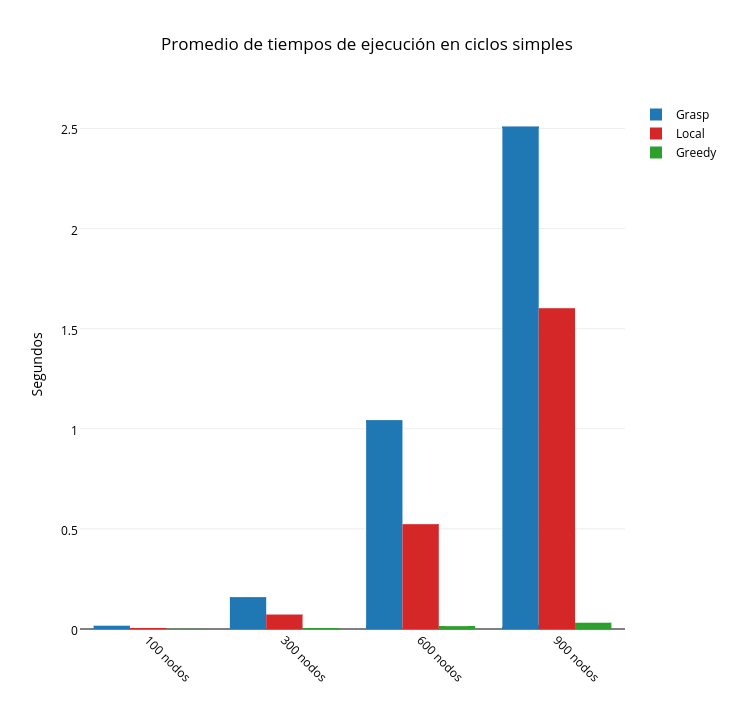
\includegraphics[width=13cm, keepaspectratio=yes]{imagenes/coliseo/Cicle.png}
\end{center}

\textcolor{red}{Coronar esto diciendo quien es mejor (es decir, el que menos tarda entre los que obtienen mejores resultados en promedio)}
Analizando tanto tiempos como resultados obtenidos, concluimos que el algoritmo Local es el m\'as conveniente cuando el grafo es un ciclo, ya que obtiene resultados mucho mejores al Greedy a pesar
de ser un poco m\'as lento. Adem\'as, es mejor que Grasp tanto en tiempo de ejecuci\'on como en el resultado.
